% !TEX program = xelatex
\documentclass[11pt,a4paper]{report}

% --- Paquetes de Idioma y Estética ---
\usepackage[utf8]{inputenc}
\usepackage[spanish, es-nodecimaldot, es-noquoting, es-notilde]{babel}
\usepackage{amsmath, amssymb, amsfonts, amsthm}
\usepackage{geometry}
\geometry{margin=2.5cm}
\usepackage{listings}
\usepackage{xcolor}
\usepackage{hyperref}
\usepackage{graphicx}
\usepackage{newunicodechar}
% Mapeo de caracteres griegos a comandos LaTeX
\newunicodechar{θ}{\ensuremath{\theta}}
\newunicodechar{α}{\ensuremath{\alpha}}
\newunicodechar{β}{\ensuremath{\beta}}
\usepackage{csquotes}
\usepackage{tikz}
\usetikzlibrary{calc}
\usetikzlibrary{arrows.meta}
\lstset{
  extendedchars=true,
  literate={ó}{{\'o}}1 {á}{{\'a}}1 {é}{{\'e}}1 {í}{{\'i}}1 {ú}{{\'u}}1 {ñ}{{\~n}}1
}
% Configuración de colores para código
\definecolor{codegreen}{rgb}{0,0.6,0}
\definecolor{codegray}{rgb}{0.5,0.5,0.5}
\definecolor{codepurple}{rgb}{0.58,0,0.82}
\definecolor{backcolour}{rgb}{0.95,0.95,0.92}

\lstdefinestyle{mystyle}{
    backgroundcolor=\color{backcolour},   
    commentstyle=\color{codegreen},
    keywordstyle=\color{magenta},
    numberstyle=\tiny\color{codegray},
    stringstyle=\color{codepurple},
    basicstyle=\ttfamily\footnotesize, % Fuente tipo terminal
    breakatwhitespace=false,         
    breaklines=true,                 
    captionpos=b,                    
    keepspaces=true,                 
    numbers=left,                    % Números de línea a la izquierda
    numbersep=5pt,                  
    showspaces=false,                
    showstringspaces=false,
    showtabs=false,                  
    tabsize=2
}
% --- CONFIGURACIÓN TCOLORBOX ROBUSTA ---
\usepackage[most]{tcolorbox} % 'most' carga skins, breakable y otros automáticamente
\tcbuselibrary{breakable}    % Refuerzo por seguridad

\lstset{style=mystyle}
% --- Configuración de Código Python (Estilo Moderno) ---
\definecolor{codegreen}{rgb}{0,0.6,0}
\definecolor{codegray}{rgb}{0.5,0.5,0.5}
\definecolor{codepurple}{rgb}{0.58,0,0.82}
\definecolor{backcolour}{rgb}{0.97,0.97,0.98}
%\usepackage[most]{tcolorbox}

\lstset{
    language=Python,
    backgroundcolor=\color{backcolour},   
    commentstyle=\color{codegreen},
    keywordstyle=\color{blue},
    numberstyle=\tiny\color{codegray},
    stringstyle=\color{codepurple},
    basicstyle=\ttfamily\small,
    breaklines=true,                 
    captionpos=b,                    
    showstringspaces=false,
    frame=single,
    rulecolor=\color{gray!30}
}


% Caja APPBOX (Azul) - Versión compatible
\newtcolorbox{appbox}[1]{
    colback=blue!5!white,
    colframe=blue!75!black,
    fonttitle=\bfseries,
    title=Aplicación: #1,
    enhanced,      
    breakable      % Esto es lo único vital para cortar páginas
}

% --- Definición de Estilo para la Consola de Salida ---
\definecolor{terminalbg}{rgb}{0.96, 0.96, 0.94} % Gris muy suave/cálido
\definecolor{terminalframe}{rgb}{0.7, 0.7, 0.7} % Borde gris discreto

% Asegúrate de tener esto arriba: \usepackage[most]{tcolorbox}

% --- Definición de Estilo para la Consola de Salida ---
\definecolor{terminalbg}{rgb}{0.96, 0.96, 0.94} 
\definecolor{terminalframe}{rgb}{0.7, 0.7, 0.7} 

% Definición de colores (si no los tienes ya)
\definecolor{terminalbg}{rgb}{0.96, 0.96, 0.94} 
\definecolor{terminalframe}{rgb}{0.7, 0.7, 0.7} 

% CAJA ESTÁNDAR (Sin librerías complejas)
\newtcolorbox{salida}{
    colback=terminalbg,       
    colframe=terminalframe,   
    boxrule=0.5pt,            
    arc=3pt,                  
    left=6pt, right=6pt, top=4pt, bottom=4pt, 
    fontupper=\ttfamily\footnotesize\color{black!85}, 
    % --- AQUÍ ESTABA EL ERROR ---
    title=\textbf{\texttt{>\_ Output / Consola}}, % Nota el \_
    % -----------------------------
    coltitle=black!80,        
    colbacktitle=gray!15,     
    toptitle=2pt, bottomtitle=2pt, 
}
% --- DEFINICIÓN DE ALERTBLOCK PERSONALIZADO ---
% Creamos un entorno que imita al de Beamer pero para libros
\newtcolorbox{alertblock}[1]{
  colback=red!5!white,      % Fondo rojo muy suave
  colframe=red!75!black,    % Borde rojo oscuro
  fonttitle=\bfseries,      % Título en negrita
  title={#1},               % El título que le pases
  sharp corners=south,      % Esquinas de abajo rectas (opcional)
  boxrule=0.5mm,            % Grosor del borde
  arc=3mm                   % Redondeo de esquinas superiores
}
\begin{document}

% --- INICIO DE LA PORTADA ---
\begin{titlepage}
    \centering
    \vspace*{1cm}
    
    % Título del libro
    {\Huge\bfseries Matemáticas para la \par}
    \vspace{0.5cm}
    {\Huge\bfseries Inteligencia Artificial Agroambiental \par}
    
    \vspace{1.5cm}
    
    % Subtítulo
    {\Large\itshape Vectores, Matrices y Tensores con aplicaciones en Python \par}
    
    \vspace{2cm}
    
    % Autor
    {\Large \textbf{Autor:} \par}
    {\Large John Jairo Leal Gómez \par}
    
    \vfill % Empuja lo siguiente hacia el fondo de la página
    
    % Institución y Fecha
    {\large Universidad Nacional de Colombia \par}
    {\large \today \par} % Pone la fecha de hoy automáticamente
\end{titlepage}
% --- FIN DE LA PORTADA ---

% --- ESTRUCTURA DEL LIBRO ---

\pagenumbering{roman} % Activa numeración romana (i, ii, iii)
\tableofcontents      % Genera el índice
\newpage              % Obliga a saltar de página después del índice

\pagenumbering{arabic} % Reinicia a números normales (1, 2, 3)
% A partir de aquí van tus capítulos o secciones:
% \section{Estructuras de datos: escalares, vectores, matrices y tensores}

\subsection{Escalar (Rango 0)}

Un \textbf{escalar} es un número real que representa una cantidad simple, sin dirección ni estructura interna. En ciencia de datos, los escalares suelen ser hiperparámetros, métricas de desempeño o mediciones puntuales.

\textbf{Ejemplos:}
\begin{itemize}
    \item La tasa de aprendizaje en un modelo de predicción de rendimiento: $\eta = 0{,}01$,
    \item El error cuadrático medio (MSE) de un modelo de predicción de peso animal: $\text{MSE} = 4{,}3$,
    \item La humedad del suelo en un punto específico: $28{,}5\%$,
    \item La concentración horaria de $\mathrm{PM}_{2.5}$ en una estación ambiental: $32{,}7\ \mu\text{g/m}^3$,
    \item El presupuesto total asignado a un programa de sostenibilidad: $1{,}25$ millones de pesos.
\end{itemize}

\subsection{Vector (Rango 1)}
Un \textbf{vector} es una lista ordenada de números que describe un objeto o fenómeno mediante múltiples atributos medibles. Cada componente corresponde a una variable relevante en el contexto de análisis.

\textbf{Ejemplos:}
\begin{itemize}
    \item \textbf{Agronómico:} $\mathbf{x} = (120, 50, 3, 6{,}2)^\top$ → (N, P, K en kg/ha; pH del suelo)\footnote{$\mathbf{x} = (120, 50, 3, 6{,}2)^\top$ Significa que el vector es columna, y lo hemos escrito como fila},
    \item \textbf{Zootécnico:} $\mathbf{x} = (650, 3{,}8, 42, 18)^\top$ → (peso en kg, producción lechera en L/día, \% grasa, edad en meses),
    \item \textbf{Agroindustrial:} $\mathbf{x} = (85, 120, 0{,}45)^\top$ → (temperatura del horno en °C, tiempo de cocción en min, humedad final del producto),
    \item \textbf{Ambiental:} $\mathbf{x} = (45, 28, 32, 65, 1{,}2)^\top$ → ($\mathrm{PM}_{10}$, $\mathrm{PM}_{2.5}$, $\mathrm{NO}_2$, $\mathrm{O}_3$, $\mathrm{CO}$ en $\mu\text{g/m}^3$),
    \item \textbf{Administrativo:} $\mathbf{x} = (320, 95, 210, 75)^\top$ → (presupuesto en millones de pesos para: infraestructura, capacitación, operación, monitoreo ambiental).
\end{itemize}

Los vectores son la unidad básica de representación en modelos de aprendizaje automático, ya que permiten tratar cada observación como un punto en un espacio multidimensional.

\subsection{Matriz (Rango 2)}

Una \textbf{matriz} es un arreglo rectangular de números reales ordenados en filas y columnas. Si bien visualmente se asemeja a una tabla, en álgebra lineal aplicada y ciencia de datos posee una \textbf{dualidad fundamental}:

\begin{enumerate}
    \item \textbf{Como estructura de datos (Estática):} Es un contenedor donde las filas suelen representar observaciones (ej. pacientes, plantas, transacciones) y las columnas variables (ej. edad, altura, costo).
    \item \textbf{Como operador (Dinámica):} Representa una \textit{transformación lineal} que actúa sobre vectores, capaz de rotar, escalar o proyectar datos en el espacio geométrico.
\end{enumerate}

\paragraph{Definición formal}
Una matriz $\mathbf{A}$ de dimensiones $m \times n$ es un elemento del espacio vectorial $\mathbb{R}^{m \times n}$. Se denota explícitamente como:

\[
\mathbf{A} = 
\begin{pmatrix}
a_{11} & a_{12} & \cdots & a_{1n} \\
a_{21} & a_{22} & \cdots & a_{2n} \\
\vdots & \vdots & \ddots & \vdots \\
a_{m1} & a_{m2} & \cdots & a_{mn}
\end{pmatrix}_{m\times n}
\in \mathbb{R}^{m \times n}.
\]

Donde:
\begin{itemize}
    \item $m$ es el número de \textbf{filas} (eje 0 en librerías como NumPy o PyTorch).
    \item $n$ es el número de \textbf{columnas} (eje 1).
    \item $a_{ij} \in \mathbb{R}$ es la entrada escalar ubicada en la fila $i$ y columna $j$.
\end{itemize}

\subsubsection{Descomposición en Vectores: Filas vs. Columnas}

Para entender las operaciones matriciales en IA, es crucial no ver la matriz como un bloque sólido, sino como una colección de vectores.

\paragraph{1. Visión por Columnas (Espacio de Características)}
Podemos ver a $\mathbf{A}$ como una colección de $n$ vectores columna verticales. Esta visión es útil en álgebra lineal para entender conceptos como \textit{independencia lineal} o \textit{bases}.

\[
\mathbf{A} = 
\begin{pmatrix}
| & | & & | \\
\mathbf{c}_1 & \mathbf{c}_2 & \cdots & \mathbf{c}_n \\
| & | & & |
\end{pmatrix}, 
\quad \text{donde } \mathbf{c}_j \in \mathbb{R}^m.
\]

\paragraph{2. Visión por Filas (Espacio de Muestras)}
Podemos ver a $\mathbf{A}$ como una pila de $m$ vectores fila horizontales. Esta es la visión estándar en \textbf{Data Science}, donde cada fila es un objeto de estudio.

\[
\mathbf{A} = 
\begin{pmatrix}
\text{---} & \mathbf{r}_1 & \text{---} \\
\text{---} & \mathbf{r}_2 & \text{---} \\
 & \vdots & \\
\text{---} & \mathbf{r}_m & \text{---}
\end{pmatrix}, 
\quad \text{donde } \mathbf{r}_i \in \mathbb{R}^{1 \times n}.
\]

\subsubsection{La Matriz como Dataset: Ejemplo Agronómico}

Considere un estudio de suelos con 100 muestras ($m=100$) y 5 variables químicas ($n=5$). La matriz de datos $\mathbf{X} \in \mathbb{R}^{100 \times 5}$ se estructura de la siguiente forma, donde cada fila es una``foto química'' de una parcela distinta:

\[
\mathbf{X} = 
\begin{array}{c|ccccc}
 & \text{N} & \text{P} & \text{K} & \text{pH} & \text{M.O.} \\ \hline
\text{Muestra 1} & 110 & 45 & 2{,}8 & 6{,}1 & 3{,}5 \\
\text{Muestra 2} & 130 & 55 & 3{,}1 & 6{,}3 & 4{,}1 \\
\vdots & \vdots & \vdots & \vdots & \vdots & \vdots \\
\text{Muestra 100} & 100 & 50 & 2{,}9 & 5{,}9 & 3{,}2
\end{array}
\]

En este contexto, el álgebra lineal nos permite operar sobre todo el conjunto de datos simultáneamente (por ejemplo, normalizar la columna del pH para todas las muestras a la vez) mediante una técnica computacional conocida como \textbf{vectorización}, evitando el uso de bucles lentos.
\subsection{Tensor: Rango \texorpdfstring{$k$}), Generalización Multidimensional}

Un \textbf{tensor} es la estructura de datos fundamental en inteligencia artificial. Matemáticamente, representa una generalización de los conceptos de escalar, vector y matriz a un espacio de $K$ dimensiones (denominadas \textit{modos} o \textit{ejes}). 

El \textbf{rango} (u \textit{orden}) de un tensor es el número de índices necesarios para localizar un elemento de forma unívoca. En términos computacionales, esto coincide con el número de dimensiones del arreglo (propiedad \texttt{.ndim} en Python).

\textbf{Jerarquía de Tensores por su Rango:}

\begin{itemize}
    \item \textbf{Rango 0 (Escalar):} Un único número $s \in \mathbb{R}$. Representa una magnitud puntual (ej. la temperatura de un invernadero).
    \item \textbf{Rango 1 (Vector):} Una lista ordenada $\mathbf{v} \in \mathbb{R}^{n_1}$. Representa una línea de datos o un perfil de atributos (ej. parámetros de suelo N, P, K).
    \item \textbf{Rango 2 (Matriz):} Una rejilla bidimensional $\mathbf{M} \in \mathbb{R}^{n_1 \times n_2}$. Estructura estándar para bases de datos tabulares (filas por columnas).
    \item \textbf{Rango 3 (Tensor de 3er orden):} Un ``cubo'' de números $\mathcal{T} \in \mathbb{R}^{n_1 \times n_2 \times n_3}$. Común en imágenes a color (Alto $\times$ Ancho $\times$ Canales RGB) como en la figura \ref{fig:tensor_vis}.
    \item \textbf{Rango 4 (Tensor de 4to orden):} Un conjunto de cubos $\mathcal{T} \in \mathbb{R}^{n_1 \times n_2 \times n_3 \times n_4}$. Estructura típica para \textit{batches} (lotes) de imágenes en redes neuronales o series temporales de mapas satelitales.
\end{itemize}



\textbf{Definición formal.} 
Un tensor de orden $K$ se define como un elemento de un espacio producto de $K$ dimensiones:

\[
\mathcal{T} \in \mathbb{R}^{d_1 \times d_2 \times \dots \times d_K}
\]

donde cada $d_i$ representa la cardinalidad (tamaño) del $i$-ésimo eje. Para acceder a una entrada específica, se requiere una tupla de $K$ índices:

\[
t_{i_1, i_2, \dots, i_K} = \mathcal{T}(i_1, i_2, \dots, i_K)
\]


\begin{quote}{Ingeniería Ambiental y Teledetección}

    El uso de tensores de rango 4 permite modelar la \textbf{dispersión espaciotemporal} de contaminantes. Los ejes representan: (1) Tiempo, (2) Latitud, (3) Longitud y (4) Tipo de contaminante ($\mathrm{PM}_{2.5}, \mathrm{O}_3$, etc.). Esta estructura es la entrada para redes neuronales recurrentes-convolucionales (ConvLSTM).
\end{quote}
%\begin{figure}[ht]
%    \centering
%    \begin{tikzpicture}[scale=0.8]
%        % Matriz (2D)
%        \begin{scope}[shift={(0,0)}]
%            \draw[thick, fill=blue!10] (0,0) rectangle (2,2);
%            \node at (1, -0.5) {Matriz (2D)};
%            \draw[step=0.5, gray!50, thin] (0,0) grid (2,2);
%        \end{scope}
        
        % Flecha
%        \draw[->, thick, gray] (2.5, 1) -- (3.5, 1);
        
        % Tensor (3D)
%        \begin{scope}[shift={(4,0)}]
            % Cara frontal
%            \draw[thick, fill=blue!10] (0,0) rectangle (2,2);
%            \draw[step=0.5, gray!50, thin] (0,0) grid (2,2);
            
            % Profundidad (Cubo)
%            \draw[thick] (0,2) -- (1,3) -- (3,3) -- (3,1) -- (2,0);
%            \draw[thick] (2,2) -- (3,3);
%            \draw[thick, fill=blue!5, opacity=0.5] (1,3) -- (3,3) -- (3,1) -- (2,0) -- (0,0) -- (0,2) -- cycle;
            
            % Capas visibles (slices)
%            \draw[thin, gray] (0.5, 2) -- (1.5, 3);
%            \draw[thin, gray] (1, 2) -- (2, 3);
%            \draw[thin, gray] (1.5, 2) -- (2.5, 3);
            
%            \node at (1.5, -0.5) {Tensor (3D)};
%            \node[anchor=west] at (3.2, 2.5) {Profundidad ($k$)};
%        \end{scope}
%    \end{tikzpicture}
%    \caption{Visualización de la evolución de una matriz a un tensor. Mientras la matriz es una hoja de cálculo, un tensor 3D es como un "libro"\ con múltiples hojas.}
%    \label{fig:tensor_vis}
%\end{figure}
\begin{figure}[h]
    \centering
    % Apuntamos al SVG. Pandoc lo entenderá perfectamente.
    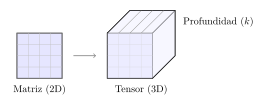
\includegraphics[width=0.8\textwidth]{images/tensor_diagrama}
    \caption{Visualización del Tensor}
\end{figure}
\subsection*{Ejemplo explícito: tensor de rango 4 en teledetección agrícola}

Considere un estudio de monitoreo de cultivos en una región agrícola mediante imágenes multiespectrales tomadas por un dron a lo largo de una temporada de crecimiento. Los datos se organizan naturalmente en un \textbf{tensor de rango 4}:

\[
\mathcal{T} \in \mathbb{R}^{30 \times 64 \times 64 \times 5}.
\]

Cada dimensión (modo) del tensor representa una característica esencial del conjunto de datos:

\begin{itemize}
    \item \textbf{Modo 1 (tiempo):} $30$ fechas de vuelo distribuidas a lo largo de la temporada (una imagen cada 3–4 días).
    \item \textbf{Modo 2 (altura):} $64$ filas de píxeles en cada imagen (resolución espacial de $64 \times 64$ píxeles por parcela).
    \item \textbf{Modo 3 (ancho):} $64$ columnas de píxeles.
    \item \textbf{Modo 4 (bandas espectrales):} $5$ bandas capturadas por el sensor multiespectral: 
    \begin{enumerate}
        \item Azul (450–515 nm),
        \item Verde (515–595 nm),
        \item Rojo (600–680 nm),
        \item Infrarrojo cercano – NIR (770–890 nm),
        \item Borde rojo – Red Edge (690–750 nm).
    \end{enumerate}
\end{itemize}

Un elemento genérico del tensor se denota como:

\[
\mathcal{T}(t, i, j, b) = \text{valor de reflectancia en la fecha } t, \text{ píxel } (i,j), \text{ y banda } b,
\]

donde:

\begin{align*}
    t &\in \{1, 2, \dots, 30\} \\
    i &\in \{1, 2, \dots, 64\} \\
    j &\in \{1, 2, \dots, 64\} \\
    b &\in \{1, 2, 3, 4, 5\}
\end{align*}

Por ejemplo, el valor $\mathcal{T}(15, 32, 45, 4) = 0.82$ indica que, en la decimoquinta fecha de muestreo, el píxel ubicado en la fila 32 y columna 45 presentó una reflectancia relativa del 82\% en la banda NIR. Este valor alto es típico de vegetación sana y se usa para calcular índices como el NDVI.

Este tipo de tensor es la entrada estándar para arquitecturas de redes neuronales convolucionales 3D (3D-CNN) o modelos basados en transformers espaciotemporales, que predicen variables como rendimiento, estrés hídrico o presencia de enfermedades a partir de la dinámica espectral y espacial del cultivo.

\textbf{Otros ejemplos prácticos con dimensiones explícitas:}

\begin{itemize}

    \item \textbf{Serie temporal de imágenes satelitales (rango 4):}  
    $\mathcal{T} \in \mathbb{R}^{36 \times 512 \times 512 \times 6}$  
    \begin{itemize}
        \item Eje 1 (36): días de observación (una imagen cada 5 días durante 180 días),
        \item Ejes 2–3 (512×512): resolución espacial de la parcela,
        \item Eje 4 (6): bandas espectrales disponibles en el satélite (e.g., Sentinel-2).  
    \end{itemize}
    Este tensor es ideal para redes neuronales recurrentes o 3D-CNN que predicen rendimiento, fenología o presencia de plagas a partir de la dinámica del cultivo.

    \item \textbf{Monitoreo de un hato lechero (rango 3):}  
    $\mathcal{T} \in \mathbb{R}^{90 \times 150 \times 4}$  
    \begin{itemize}
        \item Eje 1 (90): días de seguimiento (3 meses),
        \item Eje 2 (150): número de vacas en el hato,
        \item Eje 3 (4): variables fisiológicas: temperatura corporal, actividad (pasos), rumia (min/día), producción de leche (L/día).  
    \end{itemize}
    Este tensor permite detectar brotes de enfermedad (e.g., mastitis) mediante análisis de patrones anómalos en múltiples variables y animales simultáneamente.

    \item \textbf{Ensayo factorial en invernadero (rango 4):}  
    $\mathcal{T} \in \mathbb{R}^{5 \times 4 \times 10 \times 8}$  
    \begin{itemize}
        \item Eje 1 (5): niveles de riego,
        \item Eje 2 (4): tipos de fertilizante,
        \item Eje 3 (10): repeticiones experimentales (macetas),
        \item Eje 4 (8): variables de respuesta: altura, número de hojas, biomasa seca, contenido de nitrógeno, etc.  
    \end{itemize}
    Este tensor estructura un diseño experimental complejo y facilita el análisis multivariado de interacciones entre factores.
    \item \textbf{Secuencia de video para navegación robótica (rango 4):}  
    $\mathcal{T} \in \mathbb{R}^{30 \times 224 \times 224 \times 4}$  
    \begin{itemize}
        \item Eje 1 (30): fotogramas temporales (1 segundo de video a 30 fps),
        \item Ejes 2–3 (224×224): resolución espacial de la cámara del robot (redimensionada para una CNN),
        \item Eje 4 (4): canales de información sensorial (R, G, B y \textit{Depth}/Profundidad).  
    \end{itemize}
    
    Este tensor es la entrada típica para sistemas de \textit{Visual Servoing} o SLAM (Localización y Mapeo Simultáneos), permitiendo al robot distinguir objetos reales de sombras y calcular trayectorias libres de colisiones en entornos dinámicos.
\end{itemize}

\begin{quote}{Teledetección y Medio Ambiente}

Un tensor $\mathcal{T} \in \mathbb{R}^{30 \times 64 \times 64 \times 5}$ permite a una red neuronal convolucional (CNN) detectar estrés hídrico analizando la evolución temporal de la reflectancia en la banda NIR (Infrarrojo Cercano).
\end{quote}

En la práctica de la inteligencia artificial moderna —dominada por librerías como \texttt{PyTorch} o \texttt{TensorFlow}—, el tensor evoluciona de una abstracción matemática a un \textbf{objeto computacional} de alto rendimiento. Se implementa como un \textit{arreglo multidimensional} optimizado para ejecutarse en aceleradores de hardware (GPU/TPU) y con soporte nativo para la \textit{diferenciación automática}. Esta infraestructura es la base común que permite entrenar modelos complejos en cualquier dominio: desde la visión computacional en agricultura y la navegación robótica, hasta la proyección de escenarios financieros en administración.

\section{Manejo de los datos en Python}
A continuación, se presentan las formas para definir los datos en sus diferentes presentaciones:
\vspace{0.3cm}
\begin{lstlisting}[language=Python, caption=Implementación y Exploración de Estructuras (NumPy y PyTorch)]
import numpy as np
import torch

print("--- BLOQUE 1: CIENCIA DE DATOS (NumPy) ---")

# 1. Escalar (Rango 0)
s = 28.5 
print(f"Escalar (Humedad): {s} | Tipo: {type(s)}")

# 2. Vector (Rango 1): Perfil de suelo [N, P, K, pH]
v = np.array([120, 50, 3, 6.2])
print(f"Vector: {v} | Forma: {v.shape}")

# 3. Matriz (Rango 2): Ensayo con 3 parcelas y 2 variables (Rendimiento, pH)
M = np.array([[110, 6.1], 
              [130, 6.3], 
              [100, 5.9]])
print(f"Matriz (Parcelas x Vars):\n{M}")

# Operación de Slicing (Acceso a datos):
# "Deme el pH (columna 1) de la segunda parcela (fila 1)"
ph_parcela_2 = M[1, 1] 
print(f"--> pH de la parcela 2: {ph_parcela_2}")


print("\n--- BLOQUE 2: INTELIGENCIA ARTIFICIAL (PyTorch) ---")

# 4. Tensor Rango 3: Imagen individual para un robot (Canales, Alto, Ancho)
# PyTorch prefiere el formato (C, H, W) para procesamiento
img_robot = torch.rand(3, 128, 128) 
print(f"Imagen Robot (C,H,W): {img_robot.shape} | Rango: {img_robot.ndim}")

# 5. Tensor Rango 4: Serie de Tiempo Satelital (Multidimensional)
# Dimensiones: (Tiempo/Batch, Canales, Alto, Ancho)
# Ejemplo: 10 fechas, 5 bandas espectrales, resolución 64x64
serie_satelital = torch.randn(10, 5, 64, 64)

print(f"Serie Satelital: {serie_satelital.shape}")

# Acceso complejo: 
# "Valor del pixel central (32,32) en la Banda Roja (índice 0) de la 
# última fecha (índice -1)"
pixel_val = serie_satelital[-1, 0, 32, 32]
print(f"--> Valor pixel específico: {pixel_val:.4f}")
\end{lstlisting}
\subsection*{Salida}
\begin{salida}
--- BLOQUE 1: CIENCIA DE DATOS (NumPy) ---
Escalar (Humedad): 28.5 | Tipo: <class 'float'>

Vector: [120.  50.   3.   6.2] | Forma: (4,)

Matriz (Parcelas x Vars):
[[110.    6.1]
 [130.    6.3]
 [100.    5.9]]
--> pH de la parcela 2: 6.3

--- BLOQUE 2: INTELIGENCIA ARTIFICIAL (PyTorch) ---
Imagen Robot (C,H,W): torch.Size([3, 128, 128]) | Rango: 3

Serie Satelital: torch.Size([10, 5, 64, 64])

--> Valor pixel específico: -0.4281
\end{salida}

\section{Conceptos fundamentales de vectores en \texorpdfstring{$\mathbb{R}^n$}{Rn}}

Antes de introducir las operaciones entre vectores, es esencial comprender su estructura
interna y sus propiedades geométricas. En ciencia de datos agro-ambiental, los vectores en Rn
representan observaciones multivariadas, y su análisis requiere comprender cómo se comparan,
cómo se mide su tamaño y cómo se orientan en el espacio.

\subsection{Transpuesta de vectores y matrices}

La \textbf{transposición} es una operación fundamental que reorganiza la estructura de los datos, invirtiendo sus dimensiones: transforma un arreglo de tamaño $m \times n$ en uno de $n \times m$. Geométrica y algebraicamente, esto equivale a reflejar los elementos de la matriz respecto a su diagonal principal.

En el contexto de la ciencia de datos y la modelación, la transposición no es solo un cambio de formato, sino una herramienta indispensable para la \textbf{alineación dimensional}. Es el paso previo necesario para realizar operaciones críticas como el cálculo del producto punto, la proyección de vectores y la construcción de la \textbf{matriz de covarianza}, permitiendo así relacionar variables y observaciones de manera coherente.

\paragraph{Definición}
Dado un vector columna $\mathbf{x} \in \mathbb{R}^{n}$ (o $\mathbb{R}^{n\times 1}$), definido explícitamente como:

\[
\mathbf{x} = 
\begin{pmatrix}
x_1 \\
x_2 \\
\vdots \\
x_n
\end{pmatrix}
\]

Su \textbf{transpuesta}, denotada como $\mathbf{x}^\top$, es el vector fila asociado en $\mathbb{R}^{1 \times n}$:

\[
\mathbf{x}^\top = 
\begin{pmatrix}
x_1 & x_2 & \cdots & x_n
\end{pmatrix}
\]

\paragraph{Definición}
Dada una matriz $\mathbf{A} \in \mathbb{R}^{m \times n}$, expresada explícitamente como:

\[
\mathbf{A} = 
\begin{pmatrix}
a_{11} & a_{12} & \cdots & a_{1n} \\
a_{21} & a_{22} & \cdots & a_{2n} \\
\vdots & \vdots & \ddots & \vdots \\
a_{m1} & a_{m2} & \cdots & a_{mn}
\end{pmatrix}_{m\times n}
\]

Su \textbf{transpuesta} $\mathbf{A}^\top \in \mathbb{R}^{n \times m}$ se construye convirtiendo la fila $i$ de $\mathbf{A}$ en la columna $i$ de $\mathbf{A}^\top$:

\[
\mathbf{A}^\top = 
\begin{pmatrix}
a_{11} & a_{21} & \cdots & a_{m1} \\
a_{12} & a_{22} & \cdots & a_{m2} \\
\vdots & \vdots & \ddots & \vdots \\
a_{1n} & a_{2n} & \cdots & a_{mn}
\end{pmatrix}_{n\times m}
\]

Formalmente, se define por la propiedad de sus entradas:

\[
(\mathbf{A}^\top)_{ij} = a_{ji}, \quad \text{para todo } i=1,\dots,n,\; j=1,\dots,m.
\]


\textbf{Propiedades clave:}

\begin{align*}
    (\mathbf{A}^\top)^\top &= \mathbf{A} \\
    (\mathbf{A} + \mathbf{B})^\top &= \mathbf{A}^\top + \mathbf{B}^\top \\
    (\alpha \mathbf{A})^\top &= \alpha \mathbf{A}^\top \quad (\text{para todo } \alpha \in \mathbb{R}) \\
    (\mathbf{A} \mathbf{B})^\top &= \mathbf{B}^\top \mathbf{A}^\top \quad (\text{el orden se invierte})
\end{align*}

\paragraph{Relevancia en ciencia de datos}

\begin{itemize}
    \item \textbf{Producto punto:} El producto escalar de dos vectores columna \(\mathbf{x}, \mathbf{y} \in \mathbb{R}^n\) se escribe como \(\mathbf{x}^\top \mathbf{y}\), que resulta en un escalar. Esta notación es la base de la similitud coseno y las proyecciones.

    \item \textbf{Matriz de covarianza:} Si \(\mathbf{X} \in \mathbb{R}^{m \times n}\) es una matriz de datos (filas = observaciones, columnas = variables), la matriz de covarianza se calcula como \(\mathbf{\Sigma} = \frac{1}{m-1} \mathbf{X}^\top \mathbf{X}\). La transposición permite alinear correctamente las variables para el cálculo de covarianzas.
    \item \textbf{Ajuste de modelos:} En regresión lineal, el modelo \(\mathbf{y} = \mathbf{X} \pmb{\beta} + \pmb{\varepsilon}\) requiere que \(\mathbf{X}^\top \mathbf{X}\) sea invertible para estimar \(\pmb{\beta}\), lo que depende directamente de la transposición.

\end{itemize}

\textbf{Ejemplo numérico.}  
Considere una matriz de datos de un ensayo agronómico con 2 parcelas y 3 variables (N, P, K):

\[
\mathbf{X} =
\begin{pmatrix}
120 & 50 & 3 \\
100 & 60 & 4
\end{pmatrix}.
\]

Su transpuesta es:

\[
\mathbf{X}^\top =
\begin{pmatrix}
120 & 100 \\
50 & 60 \\
3 & 4
\end{pmatrix}.
\]

\subsection{Implementación Computacional y Matices Prácticos}

Aunque la definición matemática es estricta, en librerías como \texttt{NumPy} o \texttt{PyTorch} existe una distinción técnica importante entre un arreglo unidimensional (plano) y un vector columna formal.

\begin{itemize}
    \item \textbf{Arreglo 1D (Rank-1):} Tiene forma \texttt{(n,)}. Su transpuesta \texttt{.T} no altera nada (sigue siendo plano). Es eficiente en memoria pero peligroso en álgebra lineal estricta.
    \item \textbf{Vector Columna (Rank-2):} Tiene forma \texttt{(n, 1)}. Su transpuesta cambia la forma a \texttt{(1, n)}, comportándose exactamente como la teoría matemática.
\end{itemize}

A continuación, implementamos estos conceptos y verificamos la propiedad crítica de la inversión del producto $(\mathbf{AB})^\top = \mathbf{B}^\top \mathbf{A}^\top$.

\begin{lstlisting}[language=Python, caption=Transposición y Verificación de Propiedades en PyTorch]
import torch

print("--- 1. EL 'ENGAÑO' DE LOS VECTORES 1D ---")
# Vector plano (común en programación básica)
v_flat = torch.tensor([1, 2, 3]) 
print(f"Vector plano: {v_flat.shape}")
print(f"Transpuesta v.T: {v_flat.T.shape} (¡No cambia!)")

# Vector Matemático (Columna explícita)
# Usamos .unsqueeze(1) o definimos los corchetes dobles [[...]]
v_col = v_flat.unsqueeze(1) # Transforma (3) -> (3, 1)
print(f"Vector Columna:\n{v_col.shape}")
print(f"Vector Fila (v_col.T):\n{v_col.T.shape}")

print("\n--- 2. MATRICES Y PROPIEDAD (AB)^T ---")
# A: Matriz de datos (2 muestras, 3 variables)
A = torch.tensor([[1., 2., 3.], 
                  [4., 5., 6.]]) # Shape (2, 3)

# B: Matriz de transformación (3 entradas, 2 salidas)
B = torch.tensor([[0.1, 0.2], 
                  [0.3, 0.4], 
                  [0.5, 0.6]])   # Shape (3, 2)

# Operación: Transpuesta del producto
lhs = torch.matmul(A, B).T   # (AB)^T

# Verificación de la propiedad teórica
# INCORRECTO: A.T @ B.T (Error de dimensiones o resultado erróneo)
# CORRECTO: B.T @ A.T (Invirtiendo el orden)
rhs = torch.matmul(B.T, A.T) 

print(f"Forma de (AB).T: {lhs.shape}")
print(f"¿Es igual a B.T @ A.T?: {torch.allclose(lhs, rhs)}")
\end{lstlisting}
\subsubsection*{Salida}
\begin{salida}
--- 1. EL 'ENGAÑO' DE LOS VECTORES 1D ---
Vector plano: torch.Size([3])
Transpuesta v.T: torch.Size([3]) (¡No cambia!)
Vector Columna:
torch.Size([3, 1])
Vector Fila (v\_col.T):  % <--- AQUÍ ESTABA EL ERROR (agregué \)
torch.Size([1, 3])

--- 2. MATRICES Y PROPIEDAD (AB)\^T ---
Forma de (AB).T: torch.Size([2, 2])
¿Es igual a B.T @ A.T?: True
\end{salida}

\subsection{Transposición en Tensores (Permutación)}

Para tensores de rango $N \ge 3$, la noción de transposición se generaliza a la \textbf{permutación de ejes}. No existe una única ``transpuesta'', sino múltiples reordenamientos posibles de las dimensiones.

Dado un tensor $\mathcal{T} \in \mathbb{R}^{d_1 \times d_2 \times d_3}$, con entradas $t_{ijk}$ donde $i$ es el índice del primer eje, $j$ del segundo y $k$ del tercero.

Una permutación común (por ejemplo, invertir el orden de los ejes) genera un nuevo tensor $\mathcal{T}' \in \mathbb{R}^{d_3 \times d_2 \times d_1}$ tal que:

\[
\mathcal{T}'_{kji} = \mathcal{T}_{ijk}
\]

En la práctica de visión computacional, la operación más frecuente es intercambiar el eje de \textit{canales} (C) para moverlo del principio al final:

\textbf{Definición práctica (Cambio de Formato):}
Sea un tensor de imagen $\mathbf{I} \in \mathbb{R}^{C \times H \times W}$ (formato PyTorch). Su versión permutada $\mathbf{I}_{perm} \in \mathbb{R}^{H \times W \times C}$ (formato Matplotlib/OpenCV) se define reordenando los índices $(c, h, w) \to (h, w, c)$:

\[
\mathbf{I} = 
\left[ \text{Canales}, \text{Alto}, \text{Ancho} \right]
\xrightarrow{\text{permute}(1, 2, 0)}
\mathbf{I}_{perm} = 
\left[ \text{Alto}, \text{Ancho}, \text{Canales} \right]
\]



\begin{lstlisting}[language=Python, caption=Permutación de Ejes en PyTorch]
import torch

# Tensor 3D: Una imagen RGB simulada (3 canales, 4 alto, 4 ancho)
# Formato PyTorch: (C, H, W)
imagen_torch = torch.rand(3, 4, 4)
print(f"Forma original (C, H, W): {imagen_torch.shape}")

# PROBLEMA: Las librerías de visualización (matplotlib) esperan (H, W, C)
# SOLUCIÓN: Permutar los ejes.
# Índice 0->2 (Canales al final)
# Índice 1->0 (Alto al principio)
# Índice 2->1 (Ancho al medio)
imagen_plot = imagen_torch.permute(1, 2, 0)

print(f"Forma permutada (H, W, C): {imagen_plot.shape}")

# Cuidado: .T (transpuesta simple) en PyTorch no siempre funciona intuitivamente en tensores > 2D
# Es preferible ser explícito con .permute()
\end{lstlisting}
\subsection*{Salida}
\begin{salida}
Forma original (C, H, W): torch.Size([3, 4, 4])
Forma permutada (H, W, C): torch.Size([4, 4, 3])
\end{salida}
\subsection{Igualdad de vectores}
Dos vectores $\mathbf{x}, \mathbf{y} \in \mathbb{R}^n$ se consideran \textbf{iguales} si satisfacen simultáneamente dos condiciones:
\begin{enumerate}
    \item Pertenecen al mismo espacio vectorial (tienen la misma dimensión $n$).
    \item Sus componentes correspondientes son idénticas en valor y posición.
\end{enumerate}
Formalmente:

\[
\mathbf{x} = \mathbf{y} \quad \Longleftrightarrow \quad x_i = y_i \quad \text{para todo } i = 1, \dots, n.
\]

\paragraph{Interpretación Agronómica}
La igualdad vectorial implica una réplica exacta de condiciones. Por ejemplo, dos lotes de cultivo tienen un manejo nutricional idéntico solo si sus vectores de fertilización $\mathbf{f}_A = (N, P, K, \text{Micro})$ y $\mathbf{f}_B$ son iguales componente a componente. Si $N_A = N_B$ pero $K_A \neq K_B$, entonces $\mathbf{f}_A \neq \mathbf{f}_B$, lo que significa que los tratamientos son agronómicamente distintos.

\begin{quote}{Administración y Finanzas: Conciliación}

La igualdad vectorial es la base de la \textbf{auditoría}. Si definimos un vector de presupuesto planificado $\mathbf{p} \in \mathbb{R}^3$ y un vector de ejecución real $\mathbf{e} \in \mathbb{R}^3$ para tres departamentos (Ventas, I+D, Operaciones):

\[
\mathbf{p} = \begin{pmatrix} 100 \\ 50 \\ 80 \end{pmatrix}, \quad 
\mathbf{e} = \begin{pmatrix} 100 \\ 50 \\ 80 \end{pmatrix}
\]

La condición $\mathbf{p} = \mathbf{e}$ indica un cumplimiento presupuestario perfecto (varianza cero). Si $\mathbf{p} \neq \mathbf{e}$, la diferencia $\mathbf{d} = \mathbf{p} - \mathbf{e}$ generará un vector de desviaciones no nulo que debe ser justificado.
\end{quote}

\subsection{Igualdad de matrices}
Dos matrices $\mathbf{A}, \mathbf{B} \in \mathbb{R}^{m \times n}$ se consideran \textbf{iguales} si y solo si satisfacen simultáneamente dos condiciones:
\begin{enumerate}
    \item Tienen las mismas dimensiones (igual número de filas $m$ y columnas $n$).
    \item Sus entradas correspondientes son idénticas en valor y posición.
\end{enumerate}
Formalmente:

\[
\mathbf{A} = \mathbf{B} \quad \Longleftrightarrow \quad A_{ij} = B_{ij} \quad \text{para todo } i = 1, \dots, m; \; j = 1, \dots, n.
\]

\paragraph{Interpretación Ambiental: Detección de Cambios}
En monitoreo satelital, una imagen espectral se representa como una matriz numérica donde cada entrada corresponde a un píxel. Sea $\mathbf{M}_{2020}$ la matriz de índices de vegetación (NDVI) de una reserva forestal en 2020 y $\mathbf{M}_{2024}$ la del año actual.
La igualdad $\mathbf{M}_{2020} = \mathbf{M}_{2024}$ indicaría una conservación absoluta del ecosistema. En la práctica, los científicos buscan la matriz diferencia $\mathbf{D} = \mathbf{M}_{2024} - \mathbf{M}_{2020}$; si una entrada $D_{ij}$ es significativamente distinta de cero (negativa), alerta sobre una posible deforestación en esa coordenada específica.



\begin{quote}{Mecatrónica: Control de Robots}

En robótica, la posición y orientación de un brazo manipulador se describen mediante matrices de transformación homogénea de $4 \times 4$.
Sea $\mathbf{T}_{\text{obj}}$ la matriz que representa la pose deseada (target) del efector final (la pinza) y $\mathbf{T}_{\text{act}}$ la pose actual leída por los sensores:

\[
\mathbf{T}_{\text{obj}} = 
\begin{pmatrix} 
1 & 0 & 0 & 10 \\ 
0 & 1 & 0 & 5 \\ 
0 & 0 & 1 & 20 \\
0 & 0 & 0 & 1
\end{pmatrix}, \quad
\mathbf{T}_{\text{act}} = 
\begin{pmatrix} 
1 & 0 & 0 & 9.8 \\ 
0 & 1 & 0 & 5 \\ 
0 & 0 & 1 & 20 \\
0 & 0 & 0 & 1
\end{pmatrix}
\]

El sistema de control verifica la igualdad. Como $T_{14}$ (posición en $x$) es $10$ en la deseada y $9.8$ en la actual, $\mathbf{T}_{\text{obj}} \neq \mathbf{T}_{\text{act}}$. Esto genera una señal de error que activa los motores para corregir esa diferencia de $0.2$ unidades.
\end{quote}

\paragraph{Generalización a Tensores}
El concepto de igualdad se extiende naturalmente a arreglos multidimensionales de orden superior, conocidos como \textbf{tensores}. Sean $\mathcal{A}$ y $\mathcal{B}$ dos tensores de orden 3 (por ejemplo, de dimensiones $m \times n \times p$). Estos se consideran iguales solo si coinciden en cada voxel o celda cúbica:

\[
\mathcal{A} = \mathbf{B} \quad \Longleftrightarrow \quad A_{ijk} = B_{ijk} \quad \forall i,j,k.
\]


\subparagraph{Ejemplo: Imágenes RGB}
Una imagen digital a color se representa como un tensor de $\text{Alto} \times \text{Ancho} \times 3$ (Canales: Rojo, Verde, Azul). 
Si tenemos una imagen original $\mathcal{I}_{\text{orig}}$ y una copia transmitida por internet $\mathcal{I}_{\text{copia}}$, la igualdad $\mathcal{I}_{\text{orig}} = \mathcal{I}_{\text{copia}}$ asegura la integridad de los datos. Basta con que un solo píxel cambie levemente su tono en el canal azul para que $\mathcal{I}_{\text{orig}} \neq \mathcal{I}_{\text{copia}}$, lo cual en criptografía o esteganografía podría indicar que la imagen fue alterada.

\subsection{Igualdad Computacional: El Desafío del Punto Flotante}

En la práctica profesional de la Ciencia de Datos, rara vez verificamos la igualdad matemática estricta ($\mathbf{A} = \mathbf{B}$). Esto se debe a que las computadoras utilizan el estándar \textbf{IEEE 754} para representar números decimales (punto flotante), donde operaciones simples introducen errores infinitesimales de redondeo en los bits menos significativos.

Para abordar la comparación de tensores, es fundamental distinguir dos enfoques y una solución técnica:

\begin{enumerate}
    \item \textbf{Comparación Element-wise (Elemento a elemento):} Genera una matriz de valores booleanos del mismo tamaño que las originales. Es útil para crear ``máscaras'' y detectar \textit{dónde} difieren los datos.
    \item \textbf{Comparación Estricta:} Verifica si la estructura es idéntica en su totalidad. Falla frecuentemente con números decimales (floats).
    \item \textbf{Comparación con Tolerancia (La Solución):} Sustituye la igualdad estricta por la proximidad dentro de un umbral $\epsilon$.
\end{enumerate}

Matemáticamente, definimos la igualdad computacional como:

\[
\mathbf{A} \approx \mathbf{B} \iff |a_{ij} - b_{ij}| < \epsilon, \quad \forall i,j
\]

Donde $\epsilon$ (epsilon) suele ser un valor muy pequeño (ej. $10^{-5}$ o $10^{-8}$).

\begin{lstlisting}[language=Python, caption={El peligro de la igualdad estricta y la solución con allclose}]
import torch

print("--- 1. ELEMENT-WISE VS ESTRUCTURA ---")
A = torch.tensor([1.0, 2.0])
B = torch.tensor([1.0, 5.0]) # El segundo elemento difiere

# Comparación elemento a elemento (Genera máscara)
print(f"Máscara: {A == B}") 
# Salida esperada: [True, False]

print("\n--- 2. EL PROBLEMA DEL PUNTO FLOTANTE ---")
# Matemáticamente: (Raíz de 2) al cuadrado = 2
raiz = torch.sqrt(torch.tensor(2.0))
calculado = raiz * raiz
teorico   = torch.tensor(2.0)

# Mostramos con 10 decimales para revelar el "error fantasma"
print(f"Valor Teórico:   {teorico.item():.10f}")
print(f"Valor Calculado: {calculado.item():.10f}")

# Intento 1: Igualdad Estricta (==)
# Falla porque 2.0000000000 != 2.0000002384
print(f"¿Igualdad Estricta? {calculado == teorico}")

print("\n--- 3. SOLUCIÓN: TOLERANCIA (ALLCLOSE) ---")
# Verificamos si la diferencia es despreciable
# atol = tolerancia absoluta
es_cercano = torch.allclose(calculado, teorico, atol=1e-05)
print(f"¿Igualdad con tolerancia (allclose)? {es_cercano}")
\end{lstlisting}

\subsection*{Salida}

\begin{salida}
--- 1. ELEMENT-WISE VS ESTRUCTURA ---
Máscara: tensor([ True, False])

--- 2. EL PROBLEMA DEL PUNTO FLOTANTE ---
Valor Teórico:   2.0000000000
Valor Calculado: 2.0000002384
¿Igualdad Estricta? tensor(False)

--- 3. SOLUCIÓN: TOLERANCIA (ALLCLOSE) ---
¿Igualdad con tolerancia (allclose)? True
\end{salida}
\section{Norma euclidiana (magnitud) y dirección}

La \textbf{norma euclidiana} (también llamada longitud o módulo) de un vector $\mathbf{x} = (x_1, \dots, x_n)^\top \in \mathbb{R}^n$ se define como la raíz cuadrada de la suma de sus componentes al cuadrado:

\[
\lVert \mathbf{x} \rVert = \sqrt{x_1^2 + x_2^2 + \cdots + x_n^2} .
\]

Esta medida generaliza el concepto de distancia desde el origen hasta el punto $\mathbf{x}$. En ciencia de datos, es fundamental para normalizar variables (escalar datos), calcular el error cuadrático medio o evaluar la "fuerza" de una señal.

% --- BLOQUE 2D: TEORÍA + GRÁFICO + EJEMPLO ---
\subsubsection{Interpretación en el plano ($\mathbb{R}^2$)}
En dos dimensiones, un vector $\mathbf{x} = (x_1, x_2)^\top$ se representa geométricamente como una flecha. Sus propiedades fundamentales son:
\begin{enumerate}
    \item \textbf{Magnitud:} La longitud de la flecha, dada por Pitágoras: $\lVert \mathbf{x} \rVert = \sqrt{x_1^2 + x_2^2}$.
    \item \textbf{Dirección:} El ángulo $\theta$ respecto al eje horizontal, calculado como $\theta = \arctan(x_2 / x_1)$.
\end{enumerate}

La Figura \ref{fig:vector_componentes_norma} ilustra cómo las componentes definen tanto la posición final como la orientación del vector.

%\begin{figure}[ht]
 %   \centering
 %   \begin{tikzpicture}[scale=1.4, >=Stealth]
        % Coordenadas
%        \coordinate (O) at (0,0);
 %       \coordinate (X) at (3,2);
 %       
        % Cálculos automáticos para dibujo
%        \pgfmathsetmacro{\angle}{atan2(2,3)}
        
        % Ejes
%        \draw[->, gray!60] (-0.5,0) -- (4,0) node[right] {\small Eje 1 ($x_1$)};
%        \draw[->, gray!60] (0,-0.5) -- (0,3.0) node[above] {\small Eje 2 ($x_2$)};
        
        % Proyecciones (líneas punteadas)
%        \draw[dashed, gray] (3,0) -- (X);
%        \draw[dashed, gray] (0,2) -- (X);
        
        % Vector principal
%        \draw[->, very thick, blue] (O) -- (X);
        
        % Componentes sobre los ejes (flechas de color)
%        \draw[->, thick, blue!70] (O) -- (3,0) node[midway, below] {$x_1$};
%        \draw[->, thick, blue!70] (O) -- (0,2) node[midway, left] {$x_2$};
        
        % Ángulo theta
%        \draw[purple, thick, ->] (O) ++(0:0.8) arc[start angle=0, end angle=\angle, radius=0.8];
%        \node[purple, right] at (0.8, 0.4) {$\theta$};
        
        % Etiqueta de la norma
%        \node[blue!80, rotate=\angle, anchor=south] at ({\angle}:1.6) {\footnotesize $\lVert \mathbf{x} \rVert= \sqrt{x_1^2+x_2^2}$};
        
        % Etiqueta del vector
%        \node[blue] at (X) [above right] {$\mathbf{x}=(x_1,x_2)$};
 %   \end{tikzpicture}
 %   \caption{Representación geométrica: la norma es la longitud de la hipotenusa y $\theta$ determina la orientación.}
 %   \label{fig:vector_componentes_norma}
%\end{figure}

\begin{figure}[ht]
    \centering
    % Aquí llamamos a la imagen externa. 
    % Pandoc usará la versión .svg para web, LaTeX usará .pdf para documento.
    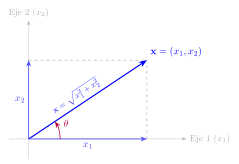
\includegraphics[width=0.7\textwidth]{images/figura_vector} 
    
    \caption{Representación geométrica: la norma es la longitud de la hipotenusa y θ determina la orientación.}
    
    % EL LABEL DEBE IR SIEMPRE DESPUÉS DEL CAPTION
    \label{fig:vector_componentes_norma} 
\end{figure}
\begin{quote}{Ejemplo Administrativo: Presupuesto Vectorial}

Considere una propuesta presupuestaria $\mathbf{p} \in \mathbb{R}^2$ (en millones de pesos) asignada a Infraestructura y Capacitación:

\[
\mathbf{p} = \begin{pmatrix} 4 \\ 3 \end{pmatrix}
\]

\begin{itemize}
    \item \textbf{Magnitud (Esfuerzo Total):} 
    $\lVert \mathbf{p} \rVert = \sqrt{4^2 + 3^2} = \sqrt{25} = 5$. El tamaño total de la inversión es 5 millones.
    
    \item \textbf{Dirección (Prioridad Estratégica):} 
    El ángulo respecto a infraestructura es $\theta = \arctan(3/4) \approx 36{,}9^\circ$.
    \begin{itemize}
        \item Si $\theta \to 0^\circ$, la prioridad es 100\% Infraestructura.
        \item Si $\theta \to 90^\circ$, la prioridad es 100\% Capacitación.
        \item Con $36{,}9^\circ$, existe un balance inclinado hacia la infraestructura.
    \end{itemize}
\end{itemize}
\end{quote}

% --- BLOQUE 3D: TEORÍA + EJEMPLO ---
\subsubsection{Orientación en el espacio ($\mathbb{R}^3$): Cosenos directores}
En tres dimensiones, un solo ángulo no basta para definir la dirección. Para un vector $\mathbf{x} = (x_1, x_2, x_3)^\top$, utilizamos los \textbf{cosenos directores}, que son los cosenos de los ángulos $(\alpha, \beta, \gamma)$ que forma el vector con cada uno de los ejes coordenados ($x, y, z$ respectivamente):

\[
\cos(\alpha) = \frac{x_1}{\lVert \mathbf{x} \rVert}, \quad
\cos(\beta)  = \frac{x_2}{\lVert \mathbf{x} \rVert}, \quad
\cos(\gamma) = \frac{x_3}{\lVert \mathbf{x} \rVert}.
\]



Estos valores oscilan entre -1 y 1. Un valor cercano a 1 indica que el vector está muy alineado con ese eje específico, dominando el comportamiento de la variable.

\begin{quote}{Ejemplo Ambiental: Calidad del Aire}

Analicemos el vector de contaminantes (en $\mu\text{g/m}^3$) de una estación urbana:

\[
\mathbf{a} = 
\begin{pmatrix}
\mathrm{PM}_{10} \\ \mathrm{NO}_2 \\ \mathrm{O}_3
\end{pmatrix} =
\begin{pmatrix}
40 \\ 30 \\ 50
\end{pmatrix}
\]

\begin{enumerate}
    \item \textbf{Magnitud (Intensidad de Contaminación):}

    \[
    \lVert \mathbf{a} \rVert = \sqrt{40^2 + 30^2 + 50^2} = \sqrt{5000} \approx 70{,}71.
    \]
    
    \item \textbf{Análisis de Dominancia (Cosenos Directores):}

    \[
    \cos(\gamma)_{\mathrm{O}_3} = \frac{50}{70{,}71} \approx \mathbf{0{,}707}, \quad
    \cos(\alpha)_{\mathrm{PM}_{10}} \approx 0{,}566.
    \]

    La componente de Ozono ($\mathrm{O}_3$) tiene el coseno director más alto ($0{,}707$), lo que indica que es el contaminante dominante en este perfil. Esto sugiere un problema de tipo fotoquímico (reacción a la luz solar) más que de emisiones primarias de combustión ($\mathrm{NO}_2$), permitiendo a las autoridades decidir si restringen el tráfico o la industria.
\end{enumerate}
\end{quote}

\subsection{Implementación Computacional: Normas y Normalización}

En el ecosistema de Python (NumPy y PyTorch), el cálculo de la magnitud y la dirección está altamente optimizado. No es necesario iterar manualmente sobre los elementos sumando cuadrados; las librerías utilizan rutinas de bajo nivel (BLAS/LAPACK) para hacerlo instantáneamente.

\subsubsection{Cálculo de la Norma ($L_2$)}
Aunque la fórmula es $\sqrt{\sum x_i^2}$, en código utilizamos funciones dedicadas como \texttt{torch.norm} o \texttt{numpy.linalg.norm}. Esto previene errores de desbordamiento numérico (overflow) cuando los números son muy grandes.

\begin{lstlisting}[language=Python, caption=Cálculo de la Magnitud (Norma Euclidiana)]
import torch

# Ejemplo Administrativo: Presupuesto [Infra, Capa]
p = torch.tensor([4.0, 3.0])

# FORMA 1: Manual (Solo con fines educativos)
# Paso a paso: Cuadrado -> Suma -> Raíz
norma_manual = torch.sqrt(torch.sum(p**2))

# FORMA 2: Profesional (La que usarás siempre)
# Es más rápida y numéricamente estable
norma_pro = torch.norm(p)

print(f"Vector p: {p}")
print(f"Norma Manual: {norma_manual.item()}") # 5.0
print(f"Norma Pro:    {norma_pro.item()}")    # 5.0
\end{lstlisting}

\subsection*{Salida}
\begin{salida}
Vector p: tensor([4., 3.])
Norma Manual: 5.0
Norma Pro:    5.0
\end{salida}

\subsubsection{Dirección y Normalización}
Aquí distinguimos entre 2D y $N$-Dimensiones:

\begin{enumerate}
    \item \textbf{En 2D (Ángulos):} No usamos $\arctan(y/x)$ porque falla si $x=0$. Usamos la función especial \texttt{atan2(y, x)}, que maneja todos los cuadrantes y la división por cero automáticamente.
    \item \textbf{En ND (Cosenos Directores = Normalización):} Calcular los cosenos directores equivale a convertir el vector en un \textbf{Vector Unitario} (longitud 1). Esta operación se llama \textbf{Normalización L2} y es vital en redes neuronales.
\end{enumerate}

\[
\hat{\mathbf{x}} = \frac{\mathbf{x}}{\lVert \mathbf{x} \rVert} = (\cos \alpha, \cos \beta, \cos \gamma)^\top
\]

\begin{lstlisting}[language=Python, caption=De la Orientación a la Normalización]
import torch
import math

print("--- 1. DIRECCIÓN EN 2D (PRESUPUESTO) ---")
p = torch.tensor([4.0, 3.0]) # x=4, y=3

# Usamos atan2(y, x). Nota: El orden es (y, x)
theta_rad = torch.atan2(p[1], p[0])

# Convertimos radianes a grados para humanos
theta_deg = torch.rad2deg(theta_rad)

print(f"Ángulo (theta): {theta_deg.item():.1f} grados")


print("\n--- 2. DIRECCIÓN EN 3D (CALIDAD AIRE) ---")
# Vector: [PM10, NO2, O3]
a = torch.tensor([40.0, 30.0, 50.0])

# Calculamos la norma
magnitud = torch.norm(a)

# Cosenos Directores: Dividimos el vector por su magnitud
# Esto crea un 'Vector Unitario' (Unit Vector)
cosenos_directores = a / magnitud

print(f"Magnitud total: {magnitud:.2f}")
print(f"Cosenos Directores (Dirección):\n{cosenos_directores}")

# Verificación: La norma de los cosenos directores siempre es 1
print(f"Comprobación (Norma del unitario): {torch.norm(cosenos_directores):.1f}")
\end{lstlisting}

\subsection*{Salida}

\begin{salida}
--- 1. DIRECCIÓN EN 2D (PRESUPUESTO) ---
Ángulo (theta): 36.9 grados

--- 2. DIRECCIÓN EN 3D (CALIDAD AIRE) ---
Magnitud total: 70.71
Cosenos Directores (Dirección):
tensor([0.5657, 0.4243, 0.7071])
Comprobación (Norma del unitario): 1.0
\end{salida}
\section{Ejercicios propuestos}

\begin{enumerate}
    \item \textbf{Clasificación de Estructuras (Rangos):}
    Identifique el rango (0, 1, 2 o $\ge 3$) y la dimensión matemática aproximada (ej. $\mathbb{R}^n$) de los siguientes objetos de datos agroambientales:
    \begin{enumerate}
        \item La concentración de nitratos en una muestra de suelo (un solo valor numérico).
        \item El perfil de temperatura de un silo medido a 10 alturas diferentes.
        \item Una fotografía aérea de un cultivo en escala de grises de $1024 \times 768$ píxeles.
        \item Un conjunto de datos multitemporal que contiene 5 bandas espectrales, para una imagen de $500 \times 500$ píxeles, tomada durante 12 meses consecutivos.
    \end{enumerate}

    \item \textbf{Interpretación de la Transpuesta:}
    Sea $\mathbf{D} \in \mathbb{R}^{100 \times 5}$ una matriz de datos donde las filas ($i=1\dots100$) representan plantas de maíz individuales y las columnas ($j=1\dots5$) representan variables medidas (Altura, Grosor de tallo, Número de hojas, Clorofila, Rendimiento).
    \begin{enumerate}
        \item ¿Cuáles son las dimensiones de la matriz transpuesta $\mathbf{D}^\top$?
        \item En la matriz $\mathbf{D}^\top$, ¿qué representa ahora una fila? ¿Y una columna?
        \item ¿Por qué podría ser útil calcular la media de las filas de $\mathbf{D}^\top$ para un análisis estadístico?
    \end{enumerate}

    \item \textbf{Verificación de Igualdad:}
    Dadas las matrices:

    \[
    \mathbf{A} = \begin{pmatrix} 1 & 2 \\ 3 & 4 \end{pmatrix}, \quad
    \mathbf{B} = \begin{pmatrix} 1 & 2 & 0 \\ 3 & 4 & 0 \end{pmatrix}, \quad
    \mathbf{C} = \begin{pmatrix} 1 & 2 \\ 3 & 4.00001 \end{pmatrix}
    \]

    \begin{enumerate}
        \item ¿Es $\mathbf{A} = \mathbf{B}$? Justifique su respuesta basándose en las dimensiones.
        \item ¿Es $\mathbf{A} = \mathbf{C}$ en términos matemáticos estrictos?
        \item Si $\mathbf{C}$ proviene de un sensor digital ruidoso, ¿consideraría estas matrices iguales en un contexto aplicado?
    \end{enumerate}

    \item \textbf{Laboratorio de Python (NumPy):}
    Escriba un script en Python que realice lo siguiente:
    \begin{itemize}
        \item Cree un vector $\mathbf{v}$ con los valores $[0, 10, 20, 30]$ (representando lecturas ideales de un sensor).
        \item Simule un vector de lectura real $\mathbf{v}_{ruido}$ sumando un pequeño valor aleatorio (ej. $0.005$) a cada componente.
        \item Intente verificar la igualdad con el operador standard \texttt{==} y comente el resultado.
        \item Verifique la igualdad correctamente utilizando \texttt{np.allclose} con una tolerancia adecuada.
    \end{itemize}

    \item \textbf{Agronómico (Análisis de Suelos - Transpuesta):} 
    Un laboratorio entrega los resultados de análisis de suelo de 3 lotes diferentes en una matriz $\mathbf{S} \in \mathbb{R}^{3 \times 4}$, donde las filas son los Lotes (A, B, C) y las columnas son los parámetros (pH, M.O., P, K).

    \[
    \mathbf{S} = 
    \begin{pmatrix}
    5.5 & 2.1 & 15 & 0.4 \\
    6.2 & 3.5 & 20 & 0.6 \\
    5.8 & 2.8 & 12 & 0.5
    \end{pmatrix}
    \]

    \begin{enumerate}
        \item Escriba explícitamente la matriz transpuesta $\mathbf{S}^\top$.
        \item Interprete el significado de la \textbf{segunda fila} de la matriz transpuesta. ¿Qué información agrupa?
    \end{enumerate}

    \item \textbf{Agrícola (Monitoreo de Cosecha - Igualdad):}
    Se tiene un vector de rendimiento estimado $\mathbf{r}_{est} = [4.5, 5.0, 4.2]^\top$ (ton/ha) para tres variedades de maíz. Al finalizar la cosecha, el vector real fue $\mathbf{r}_{real} = [4.48, 5.01, 3.8]^\top$.
    \begin{enumerate}
        \item Si definimos una tolerancia de error de $\pm 0.05$ ton/ha, ¿para cuáles variedades se cumple que $\mathbf{r}_{est} \approx \mathbf{r}_{real}$?
        \item ¿Cómo expresaría esta comparación utilizando la resta vectorial $\mathbf{d} = \mathbf{r}_{est} - \mathbf{r}_{real}$?
    \end{enumerate}

    \item \textbf{Agroindustrial (Control de Calidad - Matrices):}
    Una planta procesadora de jugos produce lotes de 3 sabores (Naranja, Mango, Mora). La matriz $\mathbf{M}_{std}$ define la formulación estándar (kg de fruta, litros de agua, kg de azúcar) y $\mathbf{M}_{lote}$ es la mezcla actual.

    \[
    \mathbf{M}_{std} = 
    \begin{pmatrix}
    100 & 50 & 5 \\
    120 & 40 & 6 \\
    90 & 60 & 4
    \end{pmatrix}
    \]

    Si el sistema de control detecta que $\mathbf{M}_{lote} \neq \mathbf{M}_{std}$, explique qué consecuencias físicas tiene esto para el producto final si la diferencia ocurre en la posición $(2,3)$ (Fila 2, Columna 3).

    \item \textbf{Ambiental (Datos Climáticos - Tensores):}
    Una estación meteorológica registra datos utilizando un tensor $\mathcal{C}$ de dimensiones $365 \times 24 \times 3$.
    \begin{itemize}
        \item Dimensión 1: Días del año ($1 \dots 365$).
        \item Dimensión 2: Horas del día ($0 \dots 23$).
        \item Dimensión 3: Variables (Temperatura, Humedad, Radiación Solar).
    \end{itemize}
    \begin{enumerate}
        \item ¿Qué representa una "rebanada" (slice) del tensor si fijamos la primera dimensión (ej. día 100) y tomamos todos los datos restantes ($100, :, :$)?
        \item Si extraemos el vector $\mathbf{v} = \mathcal{C}(:, 12, 0)$, ¿qué serie de tiempo estamos analizando?
    \end{enumerate}
    

    \item \textbf{Administrativo (Inventarios - Dimensión):}
    Una cooperativa gestiona 2 bodegas. La Bodega Norte tiene un inventario representado por el vector $\mathbf{b}_N \in \mathbb{R}^{5}$ (5 tipos de insumos). La Bodega Sur maneja 6 tipos de insumos, representada por $\mathbf{b}_S \in \mathbb{R}^{6}$.
    \begin{enumerate}
        \item ¿Es matemáticamente posible realizar la operación de comparación $\mathbf{b}_N = \mathbf{b}_S$? ¿Por qué?
        \item Desde el punto de vista administrativo, ¿qué paso previo (padding o relleno) debería realizarse para poder consolidar ambos inventarios en una sola matriz?
    \end{enumerate}
    \item \textbf{Mecatrónica (Visión Artificial para Pick-and-Place):}
    Un brazo robótico utiliza una cámara de baja resolución para identificar piezas defectuosas en una banda transportadora.
    La imagen ideal de una pieza correcta está representada por la matriz binaria $\mathbf{P}_{ideal}$ (donde 1 es metal y 0 es fondo). La cámara captura una imagen $\mathbf{P}_{cam}$ de la pieza que pasa actualmente.

    \[
    \mathbf{P}_{ideal} = 
    \begin{pmatrix}
    0 & 1 & 1 & 0 \\
    0 & 1 & 1 & 0 \\
    0 & 1 & 1 & 0 \\
    0 & 0 & 0 & 0
    \end{pmatrix}
    \quad , \quad
    \mathbf{P}_{cam} = 
    \begin{pmatrix}
    0 & 0 & 0 & 0 \\
    1 & 1 & 1 & 0 \\
    1 & 1 & 1 & 0 \\
    0 & 0 & 0 & 0
    \end{pmatrix}
    \]

    \begin{enumerate}
        \item \textbf{Pre-procesamiento (Transposición):}
        El ingeniero nota que la cámara fue montada girada $90^\circ$ respecto al modelo ideal, o la pieza llegó rotada. Calcule $\mathbf{P}_{ideal}^\top$. ¿Se cumple que $\mathbf{P}_{ideal}^\top = \mathbf{P}_{cam}$?
        
        \item \textbf{Detección de Defectos (Matrices Diferencia):}
        Suponga ahora que llega una nueva pieza $\mathbf{P}_{nueva}$. Para encontrar defectos, el robot calcula la "matriz de error" $\mathbf{E} = \mathbf{P}_{ideal} - \mathbf{P}_{nueva}$.
        Si el resultado es:

        \[
        \mathbf{E} = 
        \begin{pmatrix}
        0 & 0 & 0 & 0 \\
        0 & 1 & 0 & 0 \\
        0 & 0 & 0 & 0 \\
        0 & 0 & 0 & 0
        \end{pmatrix}
        \]

        Interprete el resultado: ¿Le falta material a la pieza o le sobra? ¿En qué coordenada específica $(i, j)$ está el defecto físico?

        \item \textbf{Lógica de Control:}
        En un script de Python para el controlador del robot, ¿por qué la siguiente condición lógica es peligrosa para la producción?
\begin{verbatim}
if imagen_camara != imagen_ideal:
    detener_linea_produccion()
\end{verbatim}
        \textit{Pista: Piense en el ruido eléctrico de los sensores o cambios de iluminación.}
    \end{enumerate}
\end{enumerate}
\paragraph{Ejercicios de Integración: Magnitud vs. Dirección}

Estos ejercicios están diseñados para distinguir cuándo un cambio en los datos es de \textit{escala} (magnitud) y cuándo es de \textit{comportamiento} (dirección).

\begin{enumerate}
    \item \textbf{Agronomía: Diagnóstico Nutricional (Colinealidad)}
    Se analizan dos muestras de suelo de lotes vecinos. Los vectores de nutrientes (Nitrógeno, Fósforo) en ppm son:

    \[ 
    \mathbf{x}_A = \begin{pmatrix} 20 \\ 10 \end{pmatrix}, \quad \mathbf{x}_B = \begin{pmatrix} 60 \\ 30 \end{pmatrix} 
    \]

    \begin{enumerate}
        \item Calcule la magnitud (riqueza total nutricional) de cada lote: $\lVert \mathbf{x}_A \rVert$ y $\lVert \mathbf{x}_B \rVert$.
        \item Calcule la dirección (ángulo $\theta$) de cada vector respecto al eje de Nitrógeno.
        \item \textbf{Interpretación:} ¿Puede afirmar que el Lote B tiene un "balance químico" diferente al Lote A, o simplemente está "más concentrado"? Justifique usando el ángulo.
    \end{enumerate}

    \item \textbf{Finanzas: Perfiles de Riesgo}
    Dos fondos de inversión distribuyen su capital en (Bonos del Estado, Acciones Tecnológicas). Los vectores en millones de USD son:

    \[ 
    \mathbf{f}_1 = \begin{pmatrix} 8 \\ 2 \end{pmatrix}, \quad \mathbf{f}_2 = \begin{pmatrix} 3 \\ 6 \end{pmatrix} 
    \]

    \begin{enumerate}
        \item ¿Qué fondo maneja mayor capital total? (Compare normas).
        \item Calcule el ángulo de cada fondo respecto al eje de "Bonos del Estado" ($x_1$).
        \item Si definimos un perfil "Conservador" como aquel con $\theta < 30^\circ$ y "Agresivo" como $\theta > 60^\circ$, clasifique a cada fondo.
    \end{enumerate}

    \item \textbf{Ingeniería/Mecatrónica: Fuerza Resultante en 3D}
    Un dron agrícola está sometido a tres fuerzas de viento representadas por el vector $\mathbf{v} = (3, 4, 12)$ m/s (componentes en $x, y, z$).
    \begin{enumerate}
        \item Calcule la velocidad total del viento (la rapidez) hallando $\lVert \mathbf{v} \rVert$. 
        \textit{(Pista: $3^2+4^2=25$ y $12^2=144$).}
        \item Calcule los cosenos directores. ¿Cuál es la componente dominante?
        \item Si el dron solo puede tolerar vientos verticales ($z$) que representen menos del 50\% de la fuerza total del viento (es decir, $\cos(\gamma) < 0.5$), ¿es seguro volar?
    \end{enumerate}

    \item \textbf{Desafío de Python: Normalización de Datos}
    En Inteligencia Artificial, a menudo necesitamos que los vectores tengan una longitud estándar de 1 (vectores unitarios) para compararlos justamente.
    Escriba un pequeño script o pseudocódigo que:
    \begin{itemize}
        \item Defina el vector $\mathbf{v} = [10, 20, 20]$.
        \item Calcule su norma $L = \lVert \mathbf{v} \rVert$.
        \item Cree un nuevo vector $\mathbf{u} = \mathbf{v} / L$.
        \item Verifique computacionalmente que la norma del nuevo vector $\mathbf{u}$ es igual a 1.
    \end{itemize}
\end{enumerate}

\chapter{El Motor de la IA: De Escalares a Tensores}

En este capítulo se presentan los conceptos preliminares de álgebra lineal necesarios para el desarrollo de modelos de inteligencia artificial en contextos agro-ambientales, industriales y administrativos.

\section{Estructuras de datos: escalares, vectores, matrices y tensores}

\subsection{Escalar (Rango 0)}

Un \textbf{escalar} es un número real que representa una cantidad simple, sin dirección ni estructura interna. En ciencia de datos, los escalares suelen ser hiperparámetros, métricas de desempeño o mediciones puntuales.

\textbf{Ejemplos:}
\begin{itemize}
    \item La tasa de aprendizaje en un modelo de predicción de rendimiento: $\eta = 0{,}01$,
    \item El error cuadrático medio (MSE) de un modelo de predicción de peso animal: $\text{MSE} = 4{,}3$,
    \item La humedad del suelo en un punto específico: $28{,}5\%$,
    \item La concentración horaria de $\mathrm{PM}_{2.5}$ en una estación ambiental: $32{,}7\ \mu\text{g/m}^3$,
    \item El presupuesto total asignado a un programa de sostenibilidad: $1{,}25$ millones de pesos.
\end{itemize}

\subsection{Vector (Rango 1)}
Un \textbf{vector} es una lista ordenada de números que describe un objeto o fenómeno mediante múltiples atributos medibles. Cada componente corresponde a una variable relevante en el contexto de análisis.

\textbf{Ejemplos:}
\begin{itemize}
    \item \textbf{Agronómico:} $\mathbf{x} = (120, 50, 3, 6{,}2)^\top$ → (N, P, K en kg/ha; pH del suelo)\footnote{$\mathbf{x} = (120, 50, 3, 6{,}2)^\top$ Significa que el vector es columna, y lo hemos escrito como fila},
    \item \textbf{Zootécnico:} $\mathbf{x} = (650, 3{,}8, 42, 18)^\top$ → (peso en kg, producción lechera en L/día, \% grasa, edad en meses),
    \item \textbf{Agroindustrial:} $\mathbf{x} = (85, 120, 0{,}45)^\top$ → (temperatura del horno en °C, tiempo de cocción en min, humedad final del producto),
    \item \textbf{Ambiental:} $\mathbf{x} = (45, 28, 32, 65, 1{,}2)^\top$ → ($\mathrm{PM}_{10}$, $\mathrm{PM}_{2.5}$, $\mathrm{NO}_2$, $\mathrm{O}_3$, $\mathrm{CO}$ en $\mu\text{g/m}^3$),
    \item \textbf{Administrativo:} $\mathbf{x} = (320, 95, 210, 75)^\top$ → (presupuesto en millones de pesos para: infraestructura, capacitación, operación, monitoreo ambiental).
\end{itemize}

Los vectores son la unidad básica de representación en modelos de aprendizaje automático, ya que permiten tratar cada observación como un punto en un espacio multidimensional.

\subsection{Matriz (Rango 2)}

Una \textbf{matriz} es un arreglo rectangular de números reales ordenados en filas y columnas. Si bien visualmente se asemeja a una tabla, en álgebra lineal aplicada y ciencia de datos posee una \textbf{dualidad fundamental}:

\begin{enumerate}
    \item \textbf{Como estructura de datos (Estática):} Es un contenedor donde las filas suelen representar observaciones (ej. pacientes, plantas, transacciones) y las columnas variables (ej. edad, altura, costo).
    \item \textbf{Como operador (Dinámica):} Representa una \textit{transformación lineal} que actúa sobre vectores, capaz de rotar, escalar o proyectar datos en el espacio geométrico.
\end{enumerate}

\paragraph{Definición formal}
Una matriz $\mathbf{A}$ de dimensiones $m \times n$ es un elemento del espacio vectorial $\mathbb{R}^{m \times n}$. Se denota explícitamente como:

\[
\mathbf{A} = 
\begin{pmatrix}
a_{11} & a_{12} & \cdots & a_{1n} \\
a_{21} & a_{22} & \cdots & a_{2n} \\
\vdots & \vdots & \ddots & \vdots \\
a_{m1} & a_{m2} & \cdots & a_{mn}
\end{pmatrix}_{m\times n}
\in \mathbb{R}^{m \times n}.
\]

Donde:
\begin{itemize}
    \item $m$ es el número de \textbf{filas} (eje 0 en librerías como NumPy o PyTorch).
    \item $n$ es el número de \textbf{columnas} (eje 1).
    \item $a_{ij} \in \mathbb{R}$ es la entrada escalar ubicada en la fila $i$ y columna $j$.
\end{itemize}

\subsubsection{Descomposición en Vectores: Filas vs. Columnas}

Para entender las operaciones matriciales en IA, es crucial no ver la matriz como un bloque sólido, sino como una colección de vectores.

\paragraph{1. Visión por Columnas (Espacio de Características)}
Podemos ver a $\mathbf{A}$ como una colección de $n$ vectores columna verticales. Esta visión es útil en álgebra lineal para entender conceptos como \textit{independencia lineal} o \textit{bases}.

\[
\mathbf{A} = 
\begin{pmatrix}
| & | & & | \\
\mathbf{c}_1 & \mathbf{c}_2 & \cdots & \mathbf{c}_n \\
| & | & & |
\end{pmatrix}, 
\quad \text{donde } \mathbf{c}_j \in \mathbb{R}^m.
\]

\paragraph{2. Visión por Filas (Espacio de Muestras)}
Podemos ver a $\mathbf{A}$ como una pila de $m$ vectores fila horizontales. Esta es la visión estándar en \textbf{Data Science}, donde cada fila es un objeto de estudio.

\[
\mathbf{A} = 
\begin{pmatrix}
\text{---} & \mathbf{r}_1 & \text{---} \\
\text{---} & \mathbf{r}_2 & \text{---} \\
 & \vdots & \\
\text{---} & \mathbf{r}_m & \text{---}
\end{pmatrix}, 
\quad \text{donde } \mathbf{r}_i \in \mathbb{R}^{1 \times n}.
\]

\subsubsection{La Matriz como Dataset: Ejemplo Agronómico}

Considere un estudio de suelos con 100 muestras ($m=100$) y 5 variables químicas ($n=5$). La matriz de datos $\mathbf{X} \in \mathbb{R}^{100 \times 5}$ se estructura de la siguiente forma, donde cada fila es una``foto química'' de una parcela distinta:

\[
\mathbf{X} = 
\begin{array}{c|ccccc}
 & \text{N} & \text{P} & \text{K} & \text{pH} & \text{M.O.} \\ \hline
\text{Muestra 1} & 110 & 45 & 2{,}8 & 6{,}1 & 3{,}5 \\
\text{Muestra 2} & 130 & 55 & 3{,}1 & 6{,}3 & 4{,}1 \\
\vdots & \vdots & \vdots & \vdots & \vdots & \vdots \\
\text{Muestra 100} & 100 & 50 & 2{,}9 & 5{,}9 & 3{,}2
\end{array}
\]

En este contexto, el álgebra lineal nos permite operar sobre todo el conjunto de datos simultáneamente (por ejemplo, normalizar la columna del pH para todas las muestras a la vez) mediante una técnica computacional conocida como \textbf{vectorización}, evitando el uso de bucles lentos.
\subsection{Tensor: Rango \texorpdfstring{$k$}), Generalización Multidimensional}

Un \textbf{tensor} es la estructura de datos fundamental en inteligencia artificial. Matemáticamente, representa una generalización de los conceptos de escalar, vector y matriz a un espacio de $K$ dimensiones (denominadas \textit{modos} o \textit{ejes}). 

El \textbf{rango} (u \textit{orden}) de un tensor es el número de índices necesarios para localizar un elemento de forma unívoca. En términos computacionales, esto coincide con el número de dimensiones del arreglo (propiedad \texttt{.ndim} en Python).

\textbf{Jerarquía de Tensores por su Rango:}

\begin{itemize}
    \item \textbf{Rango 0 (Escalar):} Un único número $s \in \mathbb{R}$. Representa una magnitud puntual (ej. la temperatura de un invernadero).
    \item \textbf{Rango 1 (Vector):} Una lista ordenada $\mathbf{v} \in \mathbb{R}^{n_1}$. Representa una línea de datos o un perfil de atributos (ej. parámetros de suelo N, P, K).
    \item \textbf{Rango 2 (Matriz):} Una rejilla bidimensional $\mathbf{M} \in \mathbb{R}^{n_1 \times n_2}$. Estructura estándar para bases de datos tabulares (filas por columnas).
    \item \textbf{Rango 3 (Tensor de 3er orden):} Un ``cubo'' de números $\mathcal{T} \in \mathbb{R}^{n_1 \times n_2 \times n_3}$. Común en imágenes a color (Alto $\times$ Ancho $\times$ Canales RGB) como en la figura \ref{fig:tensor_vis}.
    \item \textbf{Rango 4 (Tensor de 4to orden):} Un conjunto de cubos $\mathcal{T} \in \mathbb{R}^{n_1 \times n_2 \times n_3 \times n_4}$. Estructura típica para \textit{batches} (lotes) de imágenes en redes neuronales o series temporales de mapas satelitales.
\end{itemize}



\textbf{Definición formal.} 
Un tensor de orden $K$ se define como un elemento de un espacio producto de $K$ dimensiones:

\[
\mathcal{T} \in \mathbb{R}^{d_1 \times d_2 \times \dots \times d_K}
\]

donde cada $d_i$ representa la cardinalidad (tamaño) del $i$-ésimo eje. Para acceder a una entrada específica, se requiere una tupla de $K$ índices:

\[
t_{i_1, i_2, \dots, i_K} = \mathcal{T}(i_1, i_2, \dots, i_K)
\]


\begin{quote}{Ingeniería Ambiental y Teledetección}

    El uso de tensores de rango 4 permite modelar la \textbf{dispersión espaciotemporal} de contaminantes. Los ejes representan: (1) Tiempo, (2) Latitud, (3) Longitud y (4) Tipo de contaminante ($\mathrm{PM}_{2.5}, \mathrm{O}_3$, etc.). Esta estructura es la entrada para redes neuronales recurrentes-convolucionales (ConvLSTM).
\end{quote}
%\begin{figure}[ht]
%    \centering
%    \begin{tikzpicture}[scale=0.8]
%        % Matriz (2D)
%        \begin{scope}[shift={(0,0)}]
%            \draw[thick, fill=blue!10] (0,0) rectangle (2,2);
%            \node at (1, -0.5) {Matriz (2D)};
%            \draw[step=0.5, gray!50, thin] (0,0) grid (2,2);
%        \end{scope}
        
        % Flecha
%        \draw[->, thick, gray] (2.5, 1) -- (3.5, 1);
        
        % Tensor (3D)
%        \begin{scope}[shift={(4,0)}]
            % Cara frontal
%            \draw[thick, fill=blue!10] (0,0) rectangle (2,2);
%            \draw[step=0.5, gray!50, thin] (0,0) grid (2,2);
            
            % Profundidad (Cubo)
%            \draw[thick] (0,2) -- (1,3) -- (3,3) -- (3,1) -- (2,0);
%            \draw[thick] (2,2) -- (3,3);
%            \draw[thick, fill=blue!5, opacity=0.5] (1,3) -- (3,3) -- (3,1) -- (2,0) -- (0,0) -- (0,2) -- cycle;
            
            % Capas visibles (slices)
%            \draw[thin, gray] (0.5, 2) -- (1.5, 3);
%            \draw[thin, gray] (1, 2) -- (2, 3);
%            \draw[thin, gray] (1.5, 2) -- (2.5, 3);
            
%            \node at (1.5, -0.5) {Tensor (3D)};
%            \node[anchor=west] at (3.2, 2.5) {Profundidad ($k$)};
%        \end{scope}
%    \end{tikzpicture}
%    \caption{Visualización de la evolución de una matriz a un tensor. Mientras la matriz es una hoja de cálculo, un tensor 3D es como un "libro"\ con múltiples hojas.}
%    \label{fig:tensor_vis}
%\end{figure}
\begin{figure}[h]
    \centering
    % Apuntamos al SVG. Pandoc lo entenderá perfectamente.
    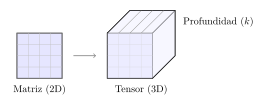
\includegraphics[width=0.8\textwidth]{images/tensor_diagrama}
    \caption{Visualización del Tensor}
\end{figure}
\subsection*{Ejemplo explícito: tensor de rango 4 en teledetección agrícola}

Considere un estudio de monitoreo de cultivos en una región agrícola mediante imágenes multiespectrales tomadas por un dron a lo largo de una temporada de crecimiento. Los datos se organizan naturalmente en un \textbf{tensor de rango 4}:

\[
\mathcal{T} \in \mathbb{R}^{30 \times 64 \times 64 \times 5}.
\]

Cada dimensión (modo) del tensor representa una característica esencial del conjunto de datos:

\begin{itemize}
    \item \textbf{Modo 1 (tiempo):} $30$ fechas de vuelo distribuidas a lo largo de la temporada (una imagen cada 3–4 días).
    \item \textbf{Modo 2 (altura):} $64$ filas de píxeles en cada imagen (resolución espacial de $64 \times 64$ píxeles por parcela).
    \item \textbf{Modo 3 (ancho):} $64$ columnas de píxeles.
    \item \textbf{Modo 4 (bandas espectrales):} $5$ bandas capturadas por el sensor multiespectral: 
    \begin{enumerate}
        \item Azul (450–515 nm),
        \item Verde (515–595 nm),
        \item Rojo (600–680 nm),
        \item Infrarrojo cercano – NIR (770–890 nm),
        \item Borde rojo – Red Edge (690–750 nm).
    \end{enumerate}
\end{itemize}

Un elemento genérico del tensor se denota como:

\[
\mathcal{T}(t, i, j, b) = \text{valor de reflectancia en la fecha } t, \text{ píxel } (i,j), \text{ y banda } b,
\]

donde:

\begin{align*}
    t &\in \{1, 2, \dots, 30\} \\
    i &\in \{1, 2, \dots, 64\} \\
    j &\in \{1, 2, \dots, 64\} \\
    b &\in \{1, 2, 3, 4, 5\}
\end{align*}

Por ejemplo, el valor $\mathcal{T}(15, 32, 45, 4) = 0.82$ indica que, en la decimoquinta fecha de muestreo, el píxel ubicado en la fila 32 y columna 45 presentó una reflectancia relativa del 82\% en la banda NIR. Este valor alto es típico de vegetación sana y se usa para calcular índices como el NDVI.

Este tipo de tensor es la entrada estándar para arquitecturas de redes neuronales convolucionales 3D (3D-CNN) o modelos basados en transformers espaciotemporales, que predicen variables como rendimiento, estrés hídrico o presencia de enfermedades a partir de la dinámica espectral y espacial del cultivo.

\textbf{Otros ejemplos prácticos con dimensiones explícitas:}

\begin{itemize}

    \item \textbf{Serie temporal de imágenes satelitales (rango 4):}  
    $\mathcal{T} \in \mathbb{R}^{36 \times 512 \times 512 \times 6}$  
    \begin{itemize}
        \item Eje 1 (36): días de observación (una imagen cada 5 días durante 180 días),
        \item Ejes 2–3 (512×512): resolución espacial de la parcela,
        \item Eje 4 (6): bandas espectrales disponibles en el satélite (e.g., Sentinel-2).  
    \end{itemize}
    Este tensor es ideal para redes neuronales recurrentes o 3D-CNN que predicen rendimiento, fenología o presencia de plagas a partir de la dinámica del cultivo.

    \item \textbf{Monitoreo de un hato lechero (rango 3):}  
    $\mathcal{T} \in \mathbb{R}^{90 \times 150 \times 4}$  
    \begin{itemize}
        \item Eje 1 (90): días de seguimiento (3 meses),
        \item Eje 2 (150): número de vacas en el hato,
        \item Eje 3 (4): variables fisiológicas: temperatura corporal, actividad (pasos), rumia (min/día), producción de leche (L/día).  
    \end{itemize}
    Este tensor permite detectar brotes de enfermedad (e.g., mastitis) mediante análisis de patrones anómalos en múltiples variables y animales simultáneamente.

    \item \textbf{Ensayo factorial en invernadero (rango 4):}  
    $\mathcal{T} \in \mathbb{R}^{5 \times 4 \times 10 \times 8}$  
    \begin{itemize}
        \item Eje 1 (5): niveles de riego,
        \item Eje 2 (4): tipos de fertilizante,
        \item Eje 3 (10): repeticiones experimentales (macetas),
        \item Eje 4 (8): variables de respuesta: altura, número de hojas, biomasa seca, contenido de nitrógeno, etc.  
    \end{itemize}
    Este tensor estructura un diseño experimental complejo y facilita el análisis multivariado de interacciones entre factores.
    \item \textbf{Secuencia de video para navegación robótica (rango 4):}  
    $\mathcal{T} \in \mathbb{R}^{30 \times 224 \times 224 \times 4}$  
    \begin{itemize}
        \item Eje 1 (30): fotogramas temporales (1 segundo de video a 30 fps),
        \item Ejes 2–3 (224×224): resolución espacial de la cámara del robot (redimensionada para una CNN),
        \item Eje 4 (4): canales de información sensorial (R, G, B y \textit{Depth}/Profundidad).  
    \end{itemize}
    
    Este tensor es la entrada típica para sistemas de \textit{Visual Servoing} o SLAM (Localización y Mapeo Simultáneos), permitiendo al robot distinguir objetos reales de sombras y calcular trayectorias libres de colisiones en entornos dinámicos.
\end{itemize}

\begin{quote}{Teledetección y Medio Ambiente}

Un tensor $\mathcal{T} \in \mathbb{R}^{30 \times 64 \times 64 \times 5}$ permite a una red neuronal convolucional (CNN) detectar estrés hídrico analizando la evolución temporal de la reflectancia en la banda NIR (Infrarrojo Cercano).
\end{quote}

En la práctica de la inteligencia artificial moderna —dominada por librerías como \texttt{PyTorch} o \texttt{TensorFlow}—, el tensor evoluciona de una abstracción matemática a un \textbf{objeto computacional} de alto rendimiento. Se implementa como un \textit{arreglo multidimensional} optimizado para ejecutarse en aceleradores de hardware (GPU/TPU) y con soporte nativo para la \textit{diferenciación automática}. Esta infraestructura es la base común que permite entrenar modelos complejos en cualquier dominio: desde la visión computacional en agricultura y la navegación robótica, hasta la proyección de escenarios financieros en administración.

\section{Manejo de los datos en Python}
A continuación, se presentan las formas para definir los datos en sus diferentes presentaciones:
\vspace{0.3cm}
\begin{lstlisting}[language=Python, caption=Implementación y Exploración de Estructuras (NumPy y PyTorch)]
import numpy as np
import torch

print("--- BLOQUE 1: CIENCIA DE DATOS (NumPy) ---")

# 1. Escalar (Rango 0)
s = 28.5 
print(f"Escalar (Humedad): {s} | Tipo: {type(s)}")

# 2. Vector (Rango 1): Perfil de suelo [N, P, K, pH]
v = np.array([120, 50, 3, 6.2])
print(f"Vector: {v} | Forma: {v.shape}")

# 3. Matriz (Rango 2): Ensayo con 3 parcelas y 2 variables (Rendimiento, pH)
M = np.array([[110, 6.1], 
              [130, 6.3], 
              [100, 5.9]])
print(f"Matriz (Parcelas x Vars):\n{M}")

# Operación de Slicing (Acceso a datos):
# "Deme el pH (columna 1) de la segunda parcela (fila 1)"
ph_parcela_2 = M[1, 1] 
print(f"--> pH de la parcela 2: {ph_parcela_2}")


print("\n--- BLOQUE 2: INTELIGENCIA ARTIFICIAL (PyTorch) ---")

# 4. Tensor Rango 3: Imagen individual para un robot (Canales, Alto, Ancho)
# PyTorch prefiere el formato (C, H, W) para procesamiento
img_robot = torch.rand(3, 128, 128) 
print(f"Imagen Robot (C,H,W): {img_robot.shape} | Rango: {img_robot.ndim}")

# 5. Tensor Rango 4: Serie de Tiempo Satelital (Multidimensional)
# Dimensiones: (Tiempo/Batch, Canales, Alto, Ancho)
# Ejemplo: 10 fechas, 5 bandas espectrales, resolución 64x64
serie_satelital = torch.randn(10, 5, 64, 64)

print(f"Serie Satelital: {serie_satelital.shape}")

# Acceso complejo: 
# "Valor del pixel central (32,32) en la Banda Roja (índice 0) de la 
# última fecha (índice -1)"
pixel_val = serie_satelital[-1, 0, 32, 32]
print(f"--> Valor pixel específico: {pixel_val:.4f}")
\end{lstlisting}
\subsection*{Salida}
\begin{salida}
--- BLOQUE 1: CIENCIA DE DATOS (NumPy) ---
Escalar (Humedad): 28.5 | Tipo: <class 'float'>

Vector: [120.  50.   3.   6.2] | Forma: (4,)

Matriz (Parcelas x Vars):
[[110.    6.1]
 [130.    6.3]
 [100.    5.9]]
--> pH de la parcela 2: 6.3

--- BLOQUE 2: INTELIGENCIA ARTIFICIAL (PyTorch) ---
Imagen Robot (C,H,W): torch.Size([3, 128, 128]) | Rango: 3

Serie Satelital: torch.Size([10, 5, 64, 64])

--> Valor pixel específico: -0.4281
\end{salida}

\section{Conceptos fundamentales de vectores en \texorpdfstring{$\mathbb{R}^n$}{Rn}}

Antes de introducir las operaciones entre vectores, es esencial comprender su estructura
interna y sus propiedades geométricas. En ciencia de datos agro-ambiental, los vectores en Rn
representan observaciones multivariadas, y su análisis requiere comprender cómo se comparan,
cómo se mide su tamaño y cómo se orientan en el espacio.

\subsection{Transpuesta de vectores y matrices}

La \textbf{transposición} es una operación fundamental que reorganiza la estructura de los datos, invirtiendo sus dimensiones: transforma un arreglo de tamaño $m \times n$ en uno de $n \times m$. Geométrica y algebraicamente, esto equivale a reflejar los elementos de la matriz respecto a su diagonal principal.

En el contexto de la ciencia de datos y la modelación, la transposición no es solo un cambio de formato, sino una herramienta indispensable para la \textbf{alineación dimensional}. Es el paso previo necesario para realizar operaciones críticas como el cálculo del producto punto, la proyección de vectores y la construcción de la \textbf{matriz de covarianza}, permitiendo así relacionar variables y observaciones de manera coherente.

\paragraph{Definición}
Dado un vector columna $\mathbf{x} \in \mathbb{R}^{n}$ (o $\mathbb{R}^{n\times 1}$), definido explícitamente como:

\[
\mathbf{x} = 
\begin{pmatrix}
x_1 \\
x_2 \\
\vdots \\
x_n
\end{pmatrix}
\]

Su \textbf{transpuesta}, denotada como $\mathbf{x}^\top$, es el vector fila asociado en $\mathbb{R}^{1 \times n}$:

\[
\mathbf{x}^\top = 
\begin{pmatrix}
x_1 & x_2 & \cdots & x_n
\end{pmatrix}
\]

\paragraph{Definición}
Dada una matriz $\mathbf{A} \in \mathbb{R}^{m \times n}$, expresada explícitamente como:

\[
\mathbf{A} = 
\begin{pmatrix}
a_{11} & a_{12} & \cdots & a_{1n} \\
a_{21} & a_{22} & \cdots & a_{2n} \\
\vdots & \vdots & \ddots & \vdots \\
a_{m1} & a_{m2} & \cdots & a_{mn}
\end{pmatrix}_{m\times n}
\]

Su \textbf{transpuesta} $\mathbf{A}^\top \in \mathbb{R}^{n \times m}$ se construye convirtiendo la fila $i$ de $\mathbf{A}$ en la columna $i$ de $\mathbf{A}^\top$:

\[
\mathbf{A}^\top = 
\begin{pmatrix}
a_{11} & a_{21} & \cdots & a_{m1} \\
a_{12} & a_{22} & \cdots & a_{m2} \\
\vdots & \vdots & \ddots & \vdots \\
a_{1n} & a_{2n} & \cdots & a_{mn}
\end{pmatrix}_{n\times m}
\]

Formalmente, se define por la propiedad de sus entradas:

\[
(\mathbf{A}^\top)_{ij} = a_{ji}, \quad \text{para todo } i=1,\dots,n,\; j=1,\dots,m.
\]


\textbf{Propiedades clave:}

\begin{align*}
    (\mathbf{A}^\top)^\top &= \mathbf{A} \\
    (\mathbf{A} + \mathbf{B})^\top &= \mathbf{A}^\top + \mathbf{B}^\top \\
    (\alpha \mathbf{A})^\top &= \alpha \mathbf{A}^\top \quad (\text{para todo } \alpha \in \mathbb{R}) \\
    (\mathbf{A} \mathbf{B})^\top &= \mathbf{B}^\top \mathbf{A}^\top \quad (\text{el orden se invierte})
\end{align*}

\paragraph{Relevancia en ciencia de datos}

\begin{itemize}
    \item \textbf{Producto punto:} El producto escalar de dos vectores columna \(\mathbf{x}, \mathbf{y} \in \mathbb{R}^n\) se escribe como \(\mathbf{x}^\top \mathbf{y}\), que resulta en un escalar. Esta notación es la base de la similitud coseno y las proyecciones.

    \item \textbf{Matriz de covarianza:} Si \(\mathbf{X} \in \mathbb{R}^{m \times n}\) es una matriz de datos (filas = observaciones, columnas = variables), la matriz de covarianza se calcula como \(\mathbf{\Sigma} = \frac{1}{m-1} \mathbf{X}^\top \mathbf{X}\). La transposición permite alinear correctamente las variables para el cálculo de covarianzas.
    \item \textbf{Ajuste de modelos:} En regresión lineal, el modelo \(\mathbf{y} = \mathbf{X} \pmb{\beta} + \pmb{\varepsilon}\) requiere que \(\mathbf{X}^\top \mathbf{X}\) sea invertible para estimar \(\pmb{\beta}\), lo que depende directamente de la transposición.

\end{itemize}

\textbf{Ejemplo numérico.}  
Considere una matriz de datos de un ensayo agronómico con 2 parcelas y 3 variables (N, P, K):

\[
\mathbf{X} =
\begin{pmatrix}
120 & 50 & 3 \\
100 & 60 & 4
\end{pmatrix}.
\]

Su transpuesta es:

\[
\mathbf{X}^\top =
\begin{pmatrix}
120 & 100 \\
50 & 60 \\
3 & 4
\end{pmatrix}.
\]

\subsection{Implementación Computacional y Matices Prácticos}

Aunque la definición matemática es estricta, en librerías como \texttt{NumPy} o \texttt{PyTorch} existe una distinción técnica importante entre un arreglo unidimensional (plano) y un vector columna formal.

\begin{itemize}
    \item \textbf{Arreglo 1D (Rank-1):} Tiene forma \texttt{(n,)}. Su transpuesta \texttt{.T} no altera nada (sigue siendo plano). Es eficiente en memoria pero peligroso en álgebra lineal estricta.
    \item \textbf{Vector Columna (Rank-2):} Tiene forma \texttt{(n, 1)}. Su transpuesta cambia la forma a \texttt{(1, n)}, comportándose exactamente como la teoría matemática.
\end{itemize}

A continuación, implementamos estos conceptos y verificamos la propiedad crítica de la inversión del producto $(\mathbf{AB})^\top = \mathbf{B}^\top \mathbf{A}^\top$.

\begin{lstlisting}[language=Python, caption=Transposición y Verificación de Propiedades en PyTorch]
import torch

print("--- 1. EL 'ENGAÑO' DE LOS VECTORES 1D ---")
# Vector plano (común en programación básica)
v_flat = torch.tensor([1, 2, 3]) 
print(f"Vector plano: {v_flat.shape}")
print(f"Transpuesta v.T: {v_flat.T.shape} (¡No cambia!)")

# Vector Matemático (Columna explícita)
# Usamos .unsqueeze(1) o definimos los corchetes dobles [[...]]
v_col = v_flat.unsqueeze(1) # Transforma (3) -> (3, 1)
print(f"Vector Columna:\n{v_col.shape}")
print(f"Vector Fila (v_col.T):\n{v_col.T.shape}")

print("\n--- 2. MATRICES Y PROPIEDAD (AB)^T ---")
# A: Matriz de datos (2 muestras, 3 variables)
A = torch.tensor([[1., 2., 3.], 
                  [4., 5., 6.]]) # Shape (2, 3)

# B: Matriz de transformación (3 entradas, 2 salidas)
B = torch.tensor([[0.1, 0.2], 
                  [0.3, 0.4], 
                  [0.5, 0.6]])   # Shape (3, 2)

# Operación: Transpuesta del producto
lhs = torch.matmul(A, B).T   # (AB)^T

# Verificación de la propiedad teórica
# INCORRECTO: A.T @ B.T (Error de dimensiones o resultado erróneo)
# CORRECTO: B.T @ A.T (Invirtiendo el orden)
rhs = torch.matmul(B.T, A.T) 

print(f"Forma de (AB).T: {lhs.shape}")
print(f"¿Es igual a B.T @ A.T?: {torch.allclose(lhs, rhs)}")
\end{lstlisting}
\subsubsection*{Salida}
\begin{salida}
--- 1. EL 'ENGAÑO' DE LOS VECTORES 1D ---
Vector plano: torch.Size([3])
Transpuesta v.T: torch.Size([3]) (¡No cambia!)
Vector Columna:
torch.Size([3, 1])
Vector Fila (v\_col.T):  % <--- AQUÍ ESTABA EL ERROR (agregué \)
torch.Size([1, 3])

--- 2. MATRICES Y PROPIEDAD (AB)\^T ---
Forma de (AB).T: torch.Size([2, 2])
¿Es igual a B.T @ A.T?: True
\end{salida}

\subsection{Transposición en Tensores (Permutación)}

Para tensores de rango $N \ge 3$, la noción de transposición se generaliza a la \textbf{permutación de ejes}. No existe una única ``transpuesta'', sino múltiples reordenamientos posibles de las dimensiones.

Dado un tensor $\mathcal{T} \in \mathbb{R}^{d_1 \times d_2 \times d_3}$, con entradas $t_{ijk}$ donde $i$ es el índice del primer eje, $j$ del segundo y $k$ del tercero.

Una permutación común (por ejemplo, invertir el orden de los ejes) genera un nuevo tensor $\mathcal{T}' \in \mathbb{R}^{d_3 \times d_2 \times d_1}$ tal que:

\[
\mathcal{T}'_{kji} = \mathcal{T}_{ijk}
\]

En la práctica de visión computacional, la operación más frecuente es intercambiar el eje de \textit{canales} (C) para moverlo del principio al final:

\textbf{Definición práctica (Cambio de Formato):}
Sea un tensor de imagen $\mathbf{I} \in \mathbb{R}^{C \times H \times W}$ (formato PyTorch). Su versión permutada $\mathbf{I}_{perm} \in \mathbb{R}^{H \times W \times C}$ (formato Matplotlib/OpenCV) se define reordenando los índices $(c, h, w) \to (h, w, c)$:

\[
\mathbf{I} = 
\left[ \text{Canales}, \text{Alto}, \text{Ancho} \right]
\xrightarrow{\text{permute}(1, 2, 0)}
\mathbf{I}_{perm} = 
\left[ \text{Alto}, \text{Ancho}, \text{Canales} \right]
\]



\begin{lstlisting}[language=Python, caption=Permutación de Ejes en PyTorch]
import torch

# Tensor 3D: Una imagen RGB simulada (3 canales, 4 alto, 4 ancho)
# Formato PyTorch: (C, H, W)
imagen_torch = torch.rand(3, 4, 4)
print(f"Forma original (C, H, W): {imagen_torch.shape}")

# PROBLEMA: Las librerías de visualización (matplotlib) esperan (H, W, C)
# SOLUCIÓN: Permutar los ejes.
# Índice 0->2 (Canales al final)
# Índice 1->0 (Alto al principio)
# Índice 2->1 (Ancho al medio)
imagen_plot = imagen_torch.permute(1, 2, 0)

print(f"Forma permutada (H, W, C): {imagen_plot.shape}")

# Cuidado: .T (transpuesta simple) en PyTorch no siempre funciona intuitivamente en tensores > 2D
# Es preferible ser explícito con .permute()
\end{lstlisting}
\subsection*{Salida}
\begin{salida}
Forma original (C, H, W): torch.Size([3, 4, 4])
Forma permutada (H, W, C): torch.Size([4, 4, 3])
\end{salida}
\subsection{Igualdad de vectores}
Dos vectores $\mathbf{x}, \mathbf{y} \in \mathbb{R}^n$ se consideran \textbf{iguales} si satisfacen simultáneamente dos condiciones:
\begin{enumerate}
    \item Pertenecen al mismo espacio vectorial (tienen la misma dimensión $n$).
    \item Sus componentes correspondientes son idénticas en valor y posición.
\end{enumerate}
Formalmente:

\[
\mathbf{x} = \mathbf{y} \quad \Longleftrightarrow \quad x_i = y_i \quad \text{para todo } i = 1, \dots, n.
\]

\paragraph{Interpretación Agronómica}
La igualdad vectorial implica una réplica exacta de condiciones. Por ejemplo, dos lotes de cultivo tienen un manejo nutricional idéntico solo si sus vectores de fertilización $\mathbf{f}_A = (N, P, K, \text{Micro})$ y $\mathbf{f}_B$ son iguales componente a componente. Si $N_A = N_B$ pero $K_A \neq K_B$, entonces $\mathbf{f}_A \neq \mathbf{f}_B$, lo que significa que los tratamientos son agronómicamente distintos.

\begin{quote}{Administración y Finanzas: Conciliación}

La igualdad vectorial es la base de la \textbf{auditoría}. Si definimos un vector de presupuesto planificado $\mathbf{p} \in \mathbb{R}^3$ y un vector de ejecución real $\mathbf{e} \in \mathbb{R}^3$ para tres departamentos (Ventas, I+D, Operaciones):

\[
\mathbf{p} = \begin{pmatrix} 100 \\ 50 \\ 80 \end{pmatrix}, \quad 
\mathbf{e} = \begin{pmatrix} 100 \\ 50 \\ 80 \end{pmatrix}
\]

La condición $\mathbf{p} = \mathbf{e}$ indica un cumplimiento presupuestario perfecto (varianza cero). Si $\mathbf{p} \neq \mathbf{e}$, la diferencia $\mathbf{d} = \mathbf{p} - \mathbf{e}$ generará un vector de desviaciones no nulo que debe ser justificado.
\end{quote}

\subsection{Igualdad de matrices}
Dos matrices $\mathbf{A}, \mathbf{B} \in \mathbb{R}^{m \times n}$ se consideran \textbf{iguales} si y solo si satisfacen simultáneamente dos condiciones:
\begin{enumerate}
    \item Tienen las mismas dimensiones (igual número de filas $m$ y columnas $n$).
    \item Sus entradas correspondientes son idénticas en valor y posición.
\end{enumerate}
Formalmente:

\[
\mathbf{A} = \mathbf{B} \quad \Longleftrightarrow \quad A_{ij} = B_{ij} \quad \text{para todo } i = 1, \dots, m; \; j = 1, \dots, n.
\]

\paragraph{Interpretación Ambiental: Detección de Cambios}
En monitoreo satelital, una imagen espectral se representa como una matriz numérica donde cada entrada corresponde a un píxel. Sea $\mathbf{M}_{2020}$ la matriz de índices de vegetación (NDVI) de una reserva forestal en 2020 y $\mathbf{M}_{2024}$ la del año actual.
La igualdad $\mathbf{M}_{2020} = \mathbf{M}_{2024}$ indicaría una conservación absoluta del ecosistema. En la práctica, los científicos buscan la matriz diferencia $\mathbf{D} = \mathbf{M}_{2024} - \mathbf{M}_{2020}$; si una entrada $D_{ij}$ es significativamente distinta de cero (negativa), alerta sobre una posible deforestación en esa coordenada específica.



\begin{quote}{Mecatrónica: Control de Robots}

En robótica, la posición y orientación de un brazo manipulador se describen mediante matrices de transformación homogénea de $4 \times 4$.
Sea $\mathbf{T}_{\text{obj}}$ la matriz que representa la pose deseada (target) del efector final (la pinza) y $\mathbf{T}_{\text{act}}$ la pose actual leída por los sensores:

\[
\mathbf{T}_{\text{obj}} = 
\begin{pmatrix} 
1 & 0 & 0 & 10 \\ 
0 & 1 & 0 & 5 \\ 
0 & 0 & 1 & 20 \\
0 & 0 & 0 & 1
\end{pmatrix}, \quad
\mathbf{T}_{\text{act}} = 
\begin{pmatrix} 
1 & 0 & 0 & 9.8 \\ 
0 & 1 & 0 & 5 \\ 
0 & 0 & 1 & 20 \\
0 & 0 & 0 & 1
\end{pmatrix}
\]

El sistema de control verifica la igualdad. Como $T_{14}$ (posición en $x$) es $10$ en la deseada y $9.8$ en la actual, $\mathbf{T}_{\text{obj}} \neq \mathbf{T}_{\text{act}}$. Esto genera una señal de error que activa los motores para corregir esa diferencia de $0.2$ unidades.
\end{quote}

\paragraph{Generalización a Tensores}
El concepto de igualdad se extiende naturalmente a arreglos multidimensionales de orden superior, conocidos como \textbf{tensores}. Sean $\mathcal{A}$ y $\mathcal{B}$ dos tensores de orden 3 (por ejemplo, de dimensiones $m \times n \times p$). Estos se consideran iguales solo si coinciden en cada voxel o celda cúbica:

\[
\mathcal{A} = \mathbf{B} \quad \Longleftrightarrow \quad A_{ijk} = B_{ijk} \quad \forall i,j,k.
\]


\subparagraph{Ejemplo: Imágenes RGB}
Una imagen digital a color se representa como un tensor de $\text{Alto} \times \text{Ancho} \times 3$ (Canales: Rojo, Verde, Azul). 
Si tenemos una imagen original $\mathcal{I}_{\text{orig}}$ y una copia transmitida por internet $\mathcal{I}_{\text{copia}}$, la igualdad $\mathcal{I}_{\text{orig}} = \mathcal{I}_{\text{copia}}$ asegura la integridad de los datos. Basta con que un solo píxel cambie levemente su tono en el canal azul para que $\mathcal{I}_{\text{orig}} \neq \mathcal{I}_{\text{copia}}$, lo cual en criptografía o esteganografía podría indicar que la imagen fue alterada.

\subsection{Igualdad Computacional: El Desafío del Punto Flotante}

En la práctica profesional de la Ciencia de Datos, rara vez verificamos la igualdad matemática estricta ($\mathbf{A} = \mathbf{B}$). Esto se debe a que las computadoras utilizan el estándar \textbf{IEEE 754} para representar números decimales (punto flotante), donde operaciones simples introducen errores infinitesimales de redondeo en los bits menos significativos.

Para abordar la comparación de tensores, es fundamental distinguir dos enfoques y una solución técnica:

\begin{enumerate}
    \item \textbf{Comparación Element-wise (Elemento a elemento):} Genera una matriz de valores booleanos del mismo tamaño que las originales. Es útil para crear ``máscaras'' y detectar \textit{dónde} difieren los datos.
    \item \textbf{Comparación Estricta:} Verifica si la estructura es idéntica en su totalidad. Falla frecuentemente con números decimales (floats).
    \item \textbf{Comparación con Tolerancia (La Solución):} Sustituye la igualdad estricta por la proximidad dentro de un umbral $\epsilon$.
\end{enumerate}

Matemáticamente, definimos la igualdad computacional como:

\[
\mathbf{A} \approx \mathbf{B} \iff |a_{ij} - b_{ij}| < \epsilon, \quad \forall i,j
\]

Donde $\epsilon$ (epsilon) suele ser un valor muy pequeño (ej. $10^{-5}$ o $10^{-8}$).

\begin{lstlisting}[language=Python, caption={El peligro de la igualdad estricta y la solución con allclose}]
import torch

print("--- 1. ELEMENT-WISE VS ESTRUCTURA ---")
A = torch.tensor([1.0, 2.0])
B = torch.tensor([1.0, 5.0]) # El segundo elemento difiere

# Comparación elemento a elemento (Genera máscara)
print(f"Máscara: {A == B}") 
# Salida esperada: [True, False]

print("\n--- 2. EL PROBLEMA DEL PUNTO FLOTANTE ---")
# Matemáticamente: (Raíz de 2) al cuadrado = 2
raiz = torch.sqrt(torch.tensor(2.0))
calculado = raiz * raiz
teorico   = torch.tensor(2.0)

# Mostramos con 10 decimales para revelar el "error fantasma"
print(f"Valor Teórico:   {teorico.item():.10f}")
print(f"Valor Calculado: {calculado.item():.10f}")

# Intento 1: Igualdad Estricta (==)
# Falla porque 2.0000000000 != 2.0000002384
print(f"¿Igualdad Estricta? {calculado == teorico}")

print("\n--- 3. SOLUCIÓN: TOLERANCIA (ALLCLOSE) ---")
# Verificamos si la diferencia es despreciable
# atol = tolerancia absoluta
es_cercano = torch.allclose(calculado, teorico, atol=1e-05)
print(f"¿Igualdad con tolerancia (allclose)? {es_cercano}")
\end{lstlisting}

\subsection*{Salida}

\begin{salida}
--- 1. ELEMENT-WISE VS ESTRUCTURA ---
Máscara: tensor([ True, False])

--- 2. EL PROBLEMA DEL PUNTO FLOTANTE ---
Valor Teórico:   2.0000000000
Valor Calculado: 2.0000002384
¿Igualdad Estricta? tensor(False)

--- 3. SOLUCIÓN: TOLERANCIA (ALLCLOSE) ---
¿Igualdad con tolerancia (allclose)? True
\end{salida}
\section{Norma euclidiana (magnitud) y dirección}

La \textbf{norma euclidiana} (también llamada longitud o módulo) de un vector $\mathbf{x} = (x_1, \dots, x_n)^\top \in \mathbb{R}^n$ se define como la raíz cuadrada de la suma de sus componentes al cuadrado:

\[
\lVert \mathbf{x} \rVert = \sqrt{x_1^2 + x_2^2 + \cdots + x_n^2} .
\]

Esta medida generaliza el concepto de distancia desde el origen hasta el punto $\mathbf{x}$. En ciencia de datos, es fundamental para normalizar variables (escalar datos), calcular el error cuadrático medio o evaluar la "fuerza" de una señal.

% --- BLOQUE 2D: TEORÍA + GRÁFICO + EJEMPLO ---
\subsubsection{Interpretación en el plano ($\mathbb{R}^2$)}
En dos dimensiones, un vector $\mathbf{x} = (x_1, x_2)^\top$ se representa geométricamente como una flecha. Sus propiedades fundamentales son:
\begin{enumerate}
    \item \textbf{Magnitud:} La longitud de la flecha, dada por Pitágoras: $\lVert \mathbf{x} \rVert = \sqrt{x_1^2 + x_2^2}$.
    \item \textbf{Dirección:} El ángulo $\theta$ respecto al eje horizontal, calculado como $\theta = \arctan(x_2 / x_1)$.
\end{enumerate}

La Figura \ref{fig:vector_componentes_norma} ilustra cómo las componentes definen tanto la posición final como la orientación del vector.

%\begin{figure}[ht]
 %   \centering
 %   \begin{tikzpicture}[scale=1.4, >=Stealth]
        % Coordenadas
%        \coordinate (O) at (0,0);
 %       \coordinate (X) at (3,2);
 %       
        % Cálculos automáticos para dibujo
%        \pgfmathsetmacro{\angle}{atan2(2,3)}
        
        % Ejes
%        \draw[->, gray!60] (-0.5,0) -- (4,0) node[right] {\small Eje 1 ($x_1$)};
%        \draw[->, gray!60] (0,-0.5) -- (0,3.0) node[above] {\small Eje 2 ($x_2$)};
        
        % Proyecciones (líneas punteadas)
%        \draw[dashed, gray] (3,0) -- (X);
%        \draw[dashed, gray] (0,2) -- (X);
        
        % Vector principal
%        \draw[->, very thick, blue] (O) -- (X);
        
        % Componentes sobre los ejes (flechas de color)
%        \draw[->, thick, blue!70] (O) -- (3,0) node[midway, below] {$x_1$};
%        \draw[->, thick, blue!70] (O) -- (0,2) node[midway, left] {$x_2$};
        
        % Ángulo theta
%        \draw[purple, thick, ->] (O) ++(0:0.8) arc[start angle=0, end angle=\angle, radius=0.8];
%        \node[purple, right] at (0.8, 0.4) {$\theta$};
        
        % Etiqueta de la norma
%        \node[blue!80, rotate=\angle, anchor=south] at ({\angle}:1.6) {\footnotesize $\lVert \mathbf{x} \rVert= \sqrt{x_1^2+x_2^2}$};
        
        % Etiqueta del vector
%        \node[blue] at (X) [above right] {$\mathbf{x}=(x_1,x_2)$};
 %   \end{tikzpicture}
 %   \caption{Representación geométrica: la norma es la longitud de la hipotenusa y $\theta$ determina la orientación.}
 %   \label{fig:vector_componentes_norma}
%\end{figure}

\begin{figure}[ht]
    \centering
    % Aquí llamamos a la imagen externa. 
    % Pandoc usará la versión .svg para web, LaTeX usará .pdf para documento.
    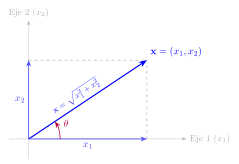
\includegraphics[width=0.7\textwidth]{images/figura_vector} 
    
    \caption{Representación geométrica: la norma es la longitud de la hipotenusa y θ determina la orientación.}
    
    % EL LABEL DEBE IR SIEMPRE DESPUÉS DEL CAPTION
    \label{fig:vector_componentes_norma} 
\end{figure}
\begin{quote}{Ejemplo Administrativo: Presupuesto Vectorial}

Considere una propuesta presupuestaria $\mathbf{p} \in \mathbb{R}^2$ (en millones de pesos) asignada a Infraestructura y Capacitación:

\[
\mathbf{p} = \begin{pmatrix} 4 \\ 3 \end{pmatrix}
\]

\begin{itemize}
    \item \textbf{Magnitud (Esfuerzo Total):} 
    $\lVert \mathbf{p} \rVert = \sqrt{4^2 + 3^2} = \sqrt{25} = 5$. El tamaño total de la inversión es 5 millones.
    
    \item \textbf{Dirección (Prioridad Estratégica):} 
    El ángulo respecto a infraestructura es $\theta = \arctan(3/4) \approx 36{,}9^\circ$.
    \begin{itemize}
        \item Si $\theta \to 0^\circ$, la prioridad es 100\% Infraestructura.
        \item Si $\theta \to 90^\circ$, la prioridad es 100\% Capacitación.
        \item Con $36{,}9^\circ$, existe un balance inclinado hacia la infraestructura.
    \end{itemize}
\end{itemize}
\end{quote}

% --- BLOQUE 3D: TEORÍA + EJEMPLO ---
\subsubsection{Orientación en el espacio ($\mathbb{R}^3$): Cosenos directores}
En tres dimensiones, un solo ángulo no basta para definir la dirección. Para un vector $\mathbf{x} = (x_1, x_2, x_3)^\top$, utilizamos los \textbf{cosenos directores}, que son los cosenos de los ángulos $(\alpha, \beta, \gamma)$ que forma el vector con cada uno de los ejes coordenados ($x, y, z$ respectivamente):

\[
\cos(\alpha) = \frac{x_1}{\lVert \mathbf{x} \rVert}, \quad
\cos(\beta)  = \frac{x_2}{\lVert \mathbf{x} \rVert}, \quad
\cos(\gamma) = \frac{x_3}{\lVert \mathbf{x} \rVert}.
\]



Estos valores oscilan entre -1 y 1. Un valor cercano a 1 indica que el vector está muy alineado con ese eje específico, dominando el comportamiento de la variable.

\begin{quote}{Ejemplo Ambiental: Calidad del Aire}

Analicemos el vector de contaminantes (en $\mu\text{g/m}^3$) de una estación urbana:

\[
\mathbf{a} = 
\begin{pmatrix}
\mathrm{PM}_{10} \\ \mathrm{NO}_2 \\ \mathrm{O}_3
\end{pmatrix} =
\begin{pmatrix}
40 \\ 30 \\ 50
\end{pmatrix}
\]

\begin{enumerate}
    \item \textbf{Magnitud (Intensidad de Contaminación):}

    \[
    \lVert \mathbf{a} \rVert = \sqrt{40^2 + 30^2 + 50^2} = \sqrt{5000} \approx 70{,}71.
    \]
    
    \item \textbf{Análisis de Dominancia (Cosenos Directores):}

    \[
    \cos(\gamma)_{\mathrm{O}_3} = \frac{50}{70{,}71} \approx \mathbf{0{,}707}, \quad
    \cos(\alpha)_{\mathrm{PM}_{10}} \approx 0{,}566.
    \]

    La componente de Ozono ($\mathrm{O}_3$) tiene el coseno director más alto ($0{,}707$), lo que indica que es el contaminante dominante en este perfil. Esto sugiere un problema de tipo fotoquímico (reacción a la luz solar) más que de emisiones primarias de combustión ($\mathrm{NO}_2$), permitiendo a las autoridades decidir si restringen el tráfico o la industria.
\end{enumerate}
\end{quote}

\subsection{Implementación Computacional: Normas y Normalización}

En el ecosistema de Python (NumPy y PyTorch), el cálculo de la magnitud y la dirección está altamente optimizado. No es necesario iterar manualmente sobre los elementos sumando cuadrados; las librerías utilizan rutinas de bajo nivel (BLAS/LAPACK) para hacerlo instantáneamente.

\subsubsection{Cálculo de la Norma ($L_2$)}
Aunque la fórmula es $\sqrt{\sum x_i^2}$, en código utilizamos funciones dedicadas como \texttt{torch.norm} o \texttt{numpy.linalg.norm}. Esto previene errores de desbordamiento numérico (overflow) cuando los números son muy grandes.

\begin{lstlisting}[language=Python, caption=Cálculo de la Magnitud (Norma Euclidiana)]
import torch

# Ejemplo Administrativo: Presupuesto [Infra, Capa]
p = torch.tensor([4.0, 3.0])

# FORMA 1: Manual (Solo con fines educativos)
# Paso a paso: Cuadrado -> Suma -> Raíz
norma_manual = torch.sqrt(torch.sum(p**2))

# FORMA 2: Profesional (La que usarás siempre)
# Es más rápida y numéricamente estable
norma_pro = torch.norm(p)

print(f"Vector p: {p}")
print(f"Norma Manual: {norma_manual.item()}") # 5.0
print(f"Norma Pro:    {norma_pro.item()}")    # 5.0
\end{lstlisting}

\subsection*{Salida}
\begin{salida}
Vector p: tensor([4., 3.])
Norma Manual: 5.0
Norma Pro:    5.0
\end{salida}

\subsubsection{Dirección y Normalización}
Aquí distinguimos entre 2D y $N$-Dimensiones:

\begin{enumerate}
    \item \textbf{En 2D (Ángulos):} No usamos $\arctan(y/x)$ porque falla si $x=0$. Usamos la función especial \texttt{atan2(y, x)}, que maneja todos los cuadrantes y la división por cero automáticamente.
    \item \textbf{En ND (Cosenos Directores = Normalización):} Calcular los cosenos directores equivale a convertir el vector en un \textbf{Vector Unitario} (longitud 1). Esta operación se llama \textbf{Normalización L2} y es vital en redes neuronales.
\end{enumerate}

\[
\hat{\mathbf{x}} = \frac{\mathbf{x}}{\lVert \mathbf{x} \rVert} = (\cos \alpha, \cos \beta, \cos \gamma)^\top
\]

\begin{lstlisting}[language=Python, caption=De la Orientación a la Normalización]
import torch
import math

print("--- 1. DIRECCIÓN EN 2D (PRESUPUESTO) ---")
p = torch.tensor([4.0, 3.0]) # x=4, y=3

# Usamos atan2(y, x). Nota: El orden es (y, x)
theta_rad = torch.atan2(p[1], p[0])

# Convertimos radianes a grados para humanos
theta_deg = torch.rad2deg(theta_rad)

print(f"Ángulo (theta): {theta_deg.item():.1f} grados")


print("\n--- 2. DIRECCIÓN EN 3D (CALIDAD AIRE) ---")
# Vector: [PM10, NO2, O3]
a = torch.tensor([40.0, 30.0, 50.0])

# Calculamos la norma
magnitud = torch.norm(a)

# Cosenos Directores: Dividimos el vector por su magnitud
# Esto crea un 'Vector Unitario' (Unit Vector)
cosenos_directores = a / magnitud

print(f"Magnitud total: {magnitud:.2f}")
print(f"Cosenos Directores (Dirección):\n{cosenos_directores}")

# Verificación: La norma de los cosenos directores siempre es 1
print(f"Comprobación (Norma del unitario): {torch.norm(cosenos_directores):.1f}")
\end{lstlisting}

\subsection*{Salida}

\begin{salida}
--- 1. DIRECCIÓN EN 2D (PRESUPUESTO) ---
Ángulo (theta): 36.9 grados

--- 2. DIRECCIÓN EN 3D (CALIDAD AIRE) ---
Magnitud total: 70.71
Cosenos Directores (Dirección):
tensor([0.5657, 0.4243, 0.7071])
Comprobación (Norma del unitario): 1.0
\end{salida}
\section{Ejercicios propuestos}

\begin{enumerate}
    \item \textbf{Clasificación de Estructuras (Rangos):}
    Identifique el rango (0, 1, 2 o $\ge 3$) y la dimensión matemática aproximada (ej. $\mathbb{R}^n$) de los siguientes objetos de datos agroambientales:
    \begin{enumerate}
        \item La concentración de nitratos en una muestra de suelo (un solo valor numérico).
        \item El perfil de temperatura de un silo medido a 10 alturas diferentes.
        \item Una fotografía aérea de un cultivo en escala de grises de $1024 \times 768$ píxeles.
        \item Un conjunto de datos multitemporal que contiene 5 bandas espectrales, para una imagen de $500 \times 500$ píxeles, tomada durante 12 meses consecutivos.
    \end{enumerate}

    \item \textbf{Interpretación de la Transpuesta:}
    Sea $\mathbf{D} \in \mathbb{R}^{100 \times 5}$ una matriz de datos donde las filas ($i=1\dots100$) representan plantas de maíz individuales y las columnas ($j=1\dots5$) representan variables medidas (Altura, Grosor de tallo, Número de hojas, Clorofila, Rendimiento).
    \begin{enumerate}
        \item ¿Cuáles son las dimensiones de la matriz transpuesta $\mathbf{D}^\top$?
        \item En la matriz $\mathbf{D}^\top$, ¿qué representa ahora una fila? ¿Y una columna?
        \item ¿Por qué podría ser útil calcular la media de las filas de $\mathbf{D}^\top$ para un análisis estadístico?
    \end{enumerate}

    \item \textbf{Verificación de Igualdad:}
    Dadas las matrices:

    \[
    \mathbf{A} = \begin{pmatrix} 1 & 2 \\ 3 & 4 \end{pmatrix}, \quad
    \mathbf{B} = \begin{pmatrix} 1 & 2 & 0 \\ 3 & 4 & 0 \end{pmatrix}, \quad
    \mathbf{C} = \begin{pmatrix} 1 & 2 \\ 3 & 4.00001 \end{pmatrix}
    \]

    \begin{enumerate}
        \item ¿Es $\mathbf{A} = \mathbf{B}$? Justifique su respuesta basándose en las dimensiones.
        \item ¿Es $\mathbf{A} = \mathbf{C}$ en términos matemáticos estrictos?
        \item Si $\mathbf{C}$ proviene de un sensor digital ruidoso, ¿consideraría estas matrices iguales en un contexto aplicado?
    \end{enumerate}

    \item \textbf{Laboratorio de Python (NumPy):}
    Escriba un script en Python que realice lo siguiente:
    \begin{itemize}
        \item Cree un vector $\mathbf{v}$ con los valores $[0, 10, 20, 30]$ (representando lecturas ideales de un sensor).
        \item Simule un vector de lectura real $\mathbf{v}_{ruido}$ sumando un pequeño valor aleatorio (ej. $0.005$) a cada componente.
        \item Intente verificar la igualdad con el operador standard \texttt{==} y comente el resultado.
        \item Verifique la igualdad correctamente utilizando \texttt{np.allclose} con una tolerancia adecuada.
    \end{itemize}

    \item \textbf{Agronómico (Análisis de Suelos - Transpuesta):} 
    Un laboratorio entrega los resultados de análisis de suelo de 3 lotes diferentes en una matriz $\mathbf{S} \in \mathbb{R}^{3 \times 4}$, donde las filas son los Lotes (A, B, C) y las columnas son los parámetros (pH, M.O., P, K).

    \[
    \mathbf{S} = 
    \begin{pmatrix}
    5.5 & 2.1 & 15 & 0.4 \\
    6.2 & 3.5 & 20 & 0.6 \\
    5.8 & 2.8 & 12 & 0.5
    \end{pmatrix}
    \]

    \begin{enumerate}
        \item Escriba explícitamente la matriz transpuesta $\mathbf{S}^\top$.
        \item Interprete el significado de la \textbf{segunda fila} de la matriz transpuesta. ¿Qué información agrupa?
    \end{enumerate}

    \item \textbf{Agrícola (Monitoreo de Cosecha - Igualdad):}
    Se tiene un vector de rendimiento estimado $\mathbf{r}_{est} = [4.5, 5.0, 4.2]^\top$ (ton/ha) para tres variedades de maíz. Al finalizar la cosecha, el vector real fue $\mathbf{r}_{real} = [4.48, 5.01, 3.8]^\top$.
    \begin{enumerate}
        \item Si definimos una tolerancia de error de $\pm 0.05$ ton/ha, ¿para cuáles variedades se cumple que $\mathbf{r}_{est} \approx \mathbf{r}_{real}$?
        \item ¿Cómo expresaría esta comparación utilizando la resta vectorial $\mathbf{d} = \mathbf{r}_{est} - \mathbf{r}_{real}$?
    \end{enumerate}

    \item \textbf{Agroindustrial (Control de Calidad - Matrices):}
    Una planta procesadora de jugos produce lotes de 3 sabores (Naranja, Mango, Mora). La matriz $\mathbf{M}_{std}$ define la formulación estándar (kg de fruta, litros de agua, kg de azúcar) y $\mathbf{M}_{lote}$ es la mezcla actual.

    \[
    \mathbf{M}_{std} = 
    \begin{pmatrix}
    100 & 50 & 5 \\
    120 & 40 & 6 \\
    90 & 60 & 4
    \end{pmatrix}
    \]

    Si el sistema de control detecta que $\mathbf{M}_{lote} \neq \mathbf{M}_{std}$, explique qué consecuencias físicas tiene esto para el producto final si la diferencia ocurre en la posición $(2,3)$ (Fila 2, Columna 3).

    \item \textbf{Ambiental (Datos Climáticos - Tensores):}
    Una estación meteorológica registra datos utilizando un tensor $\mathcal{C}$ de dimensiones $365 \times 24 \times 3$.
    \begin{itemize}
        \item Dimensión 1: Días del año ($1 \dots 365$).
        \item Dimensión 2: Horas del día ($0 \dots 23$).
        \item Dimensión 3: Variables (Temperatura, Humedad, Radiación Solar).
    \end{itemize}
    \begin{enumerate}
        \item ¿Qué representa una "rebanada" (slice) del tensor si fijamos la primera dimensión (ej. día 100) y tomamos todos los datos restantes ($100, :, :$)?
        \item Si extraemos el vector $\mathbf{v} = \mathcal{C}(:, 12, 0)$, ¿qué serie de tiempo estamos analizando?
    \end{enumerate}
    

    \item \textbf{Administrativo (Inventarios - Dimensión):}
    Una cooperativa gestiona 2 bodegas. La Bodega Norte tiene un inventario representado por el vector $\mathbf{b}_N \in \mathbb{R}^{5}$ (5 tipos de insumos). La Bodega Sur maneja 6 tipos de insumos, representada por $\mathbf{b}_S \in \mathbb{R}^{6}$.
    \begin{enumerate}
        \item ¿Es matemáticamente posible realizar la operación de comparación $\mathbf{b}_N = \mathbf{b}_S$? ¿Por qué?
        \item Desde el punto de vista administrativo, ¿qué paso previo (padding o relleno) debería realizarse para poder consolidar ambos inventarios en una sola matriz?
    \end{enumerate}
    \item \textbf{Mecatrónica (Visión Artificial para Pick-and-Place):}
    Un brazo robótico utiliza una cámara de baja resolución para identificar piezas defectuosas en una banda transportadora.
    La imagen ideal de una pieza correcta está representada por la matriz binaria $\mathbf{P}_{ideal}$ (donde 1 es metal y 0 es fondo). La cámara captura una imagen $\mathbf{P}_{cam}$ de la pieza que pasa actualmente.

    \[
    \mathbf{P}_{ideal} = 
    \begin{pmatrix}
    0 & 1 & 1 & 0 \\
    0 & 1 & 1 & 0 \\
    0 & 1 & 1 & 0 \\
    0 & 0 & 0 & 0
    \end{pmatrix}
    \quad , \quad
    \mathbf{P}_{cam} = 
    \begin{pmatrix}
    0 & 0 & 0 & 0 \\
    1 & 1 & 1 & 0 \\
    1 & 1 & 1 & 0 \\
    0 & 0 & 0 & 0
    \end{pmatrix}
    \]

    \begin{enumerate}
        \item \textbf{Pre-procesamiento (Transposición):}
        El ingeniero nota que la cámara fue montada girada $90^\circ$ respecto al modelo ideal, o la pieza llegó rotada. Calcule $\mathbf{P}_{ideal}^\top$. ¿Se cumple que $\mathbf{P}_{ideal}^\top = \mathbf{P}_{cam}$?
        
        \item \textbf{Detección de Defectos (Matrices Diferencia):}
        Suponga ahora que llega una nueva pieza $\mathbf{P}_{nueva}$. Para encontrar defectos, el robot calcula la "matriz de error" $\mathbf{E} = \mathbf{P}_{ideal} - \mathbf{P}_{nueva}$.
        Si el resultado es:

        \[
        \mathbf{E} = 
        \begin{pmatrix}
        0 & 0 & 0 & 0 \\
        0 & 1 & 0 & 0 \\
        0 & 0 & 0 & 0 \\
        0 & 0 & 0 & 0
        \end{pmatrix}
        \]

        Interprete el resultado: ¿Le falta material a la pieza o le sobra? ¿En qué coordenada específica $(i, j)$ está el defecto físico?

        \item \textbf{Lógica de Control:}
        En un script de Python para el controlador del robot, ¿por qué la siguiente condición lógica es peligrosa para la producción?
\begin{verbatim}
if imagen_camara != imagen_ideal:
    detener_linea_produccion()
\end{verbatim}
        \textit{Pista: Piense en el ruido eléctrico de los sensores o cambios de iluminación.}
    \end{enumerate}
\end{enumerate}
\paragraph{Ejercicios de Integración: Magnitud vs. Dirección}

Estos ejercicios están diseñados para distinguir cuándo un cambio en los datos es de \textit{escala} (magnitud) y cuándo es de \textit{comportamiento} (dirección).

\begin{enumerate}
    \item \textbf{Agronomía: Diagnóstico Nutricional (Colinealidad)}
    Se analizan dos muestras de suelo de lotes vecinos. Los vectores de nutrientes (Nitrógeno, Fósforo) en ppm son:

    \[ 
    \mathbf{x}_A = \begin{pmatrix} 20 \\ 10 \end{pmatrix}, \quad \mathbf{x}_B = \begin{pmatrix} 60 \\ 30 \end{pmatrix} 
    \]

    \begin{enumerate}
        \item Calcule la magnitud (riqueza total nutricional) de cada lote: $\lVert \mathbf{x}_A \rVert$ y $\lVert \mathbf{x}_B \rVert$.
        \item Calcule la dirección (ángulo $\theta$) de cada vector respecto al eje de Nitrógeno.
        \item \textbf{Interpretación:} ¿Puede afirmar que el Lote B tiene un "balance químico" diferente al Lote A, o simplemente está "más concentrado"? Justifique usando el ángulo.
    \end{enumerate}

    \item \textbf{Finanzas: Perfiles de Riesgo}
    Dos fondos de inversión distribuyen su capital en (Bonos del Estado, Acciones Tecnológicas). Los vectores en millones de USD son:

    \[ 
    \mathbf{f}_1 = \begin{pmatrix} 8 \\ 2 \end{pmatrix}, \quad \mathbf{f}_2 = \begin{pmatrix} 3 \\ 6 \end{pmatrix} 
    \]

    \begin{enumerate}
        \item ¿Qué fondo maneja mayor capital total? (Compare normas).
        \item Calcule el ángulo de cada fondo respecto al eje de "Bonos del Estado" ($x_1$).
        \item Si definimos un perfil "Conservador" como aquel con $\theta < 30^\circ$ y "Agresivo" como $\theta > 60^\circ$, clasifique a cada fondo.
    \end{enumerate}

    \item \textbf{Ingeniería/Mecatrónica: Fuerza Resultante en 3D}
    Un dron agrícola está sometido a tres fuerzas de viento representadas por el vector $\mathbf{v} = (3, 4, 12)$ m/s (componentes en $x, y, z$).
    \begin{enumerate}
        \item Calcule la velocidad total del viento (la rapidez) hallando $\lVert \mathbf{v} \rVert$. 
        \textit{(Pista: $3^2+4^2=25$ y $12^2=144$).}
        \item Calcule los cosenos directores. ¿Cuál es la componente dominante?
        \item Si el dron solo puede tolerar vientos verticales ($z$) que representen menos del 50\% de la fuerza total del viento (es decir, $\cos(\gamma) < 0.5$), ¿es seguro volar?
    \end{enumerate}

    \item \textbf{Desafío de Python: Normalización de Datos}
    En Inteligencia Artificial, a menudo necesitamos que los vectores tengan una longitud estándar de 1 (vectores unitarios) para compararlos justamente.
    Escriba un pequeño script o pseudocódigo que:
    \begin{itemize}
        \item Defina el vector $\mathbf{v} = [10, 20, 20]$.
        \item Calcule su norma $L = \lVert \mathbf{v} \rVert$.
        \item Cree un nuevo vector $\mathbf{u} = \mathbf{v} / L$.
        \item Verifique computacionalmente que la norma del nuevo vector $\mathbf{u}$ es igual a 1.
    \end{itemize}
\end{enumerate}

\chapter{Poniendo el Motor en Marcha: Aritmética Tensorial}

\section{Suma de vectores y Aplicaciones}

La suma combina dos vectores componente a componente. En términos de datos, esta operación representa la acumulación o superposición de efectos provenientes de distintas fuentes.

\textbf{Definición formal.} Sean $\mathbf{x}, \mathbf{y} \in \mathbb{R}^n$. La suma $\mathbf{x} + \mathbf{y}$ se define como:

\[
\mathbf{x} + \mathbf{y} = 
\begin{pmatrix} x_1 \\ x_2 \\ \vdots \\ x_n \end{pmatrix} + 
\begin{pmatrix} y_1 \\ y_2 \\ \vdots \\ y_n \end{pmatrix} = 
\begin{pmatrix} x_1 + y_1 \\ x_2 + y_2 \\ \vdots \\ x_n + y_n \end{pmatrix}.
\]

\begin{figure}[ht]
    \centering
    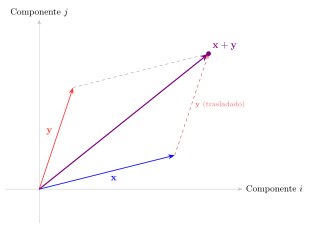
\includegraphics[width=0.8\textwidth]{images/suma_vectores}
    \caption{Representación geométrica de la suma vectorial (Ley del Paralelogramo). El vector resultante conecta el origen con la esquina opuesta formada por la proyección de los vectores $\mathbf{x}$ y $\mathbf{y}$.}
    \label{suma_vectores}
\end{figure}

Geométricamente, esto sigue la \textbf{ley del paralelogramo} \ref{suma_vectores}: si colocamos el inicio de $\mathbf{y}$ en la punta final de $\mathbf{x}$, el vector resultante va desde el origen de $\mathbf{x}$ hasta la punta final de $\mathbf{y}$.

\begin{quote}{Ejemplo Ambiental: Inventario de Emisiones}
Supongamos que en una zona industrial existen dos fuentes principales de contaminación: una Termoeléctrica ($\mathbf{e}_T$) y una Fábrica de Cemento ($\mathbf{e}_C$).
Los vectores representan la emisión diaria (en toneladas) de tres contaminantes distintos: $[\text{CO}_2, \text{NO}_x, \text{Material Particulado}]$.

\[
\mathbf{e}_T = \begin{pmatrix} 100 \\ 5 \\ 0.5 \end{pmatrix}, \quad
\mathbf{e}_C = \begin{pmatrix} 40 \\ 2 \\ 3.5 \end{pmatrix}
\]

Para conocer la \textbf{carga total} que recibe la atmósfera en esa zona, realizamos la suma vectorial:

\[
\mathbf{e}_{total} = \mathbf{e}_T + \mathbf{e}_C = 
\begin{pmatrix} 100 + 40 \\ 5 + 2 \\ 0.5 + 3.5 \end{pmatrix} = 
\begin{pmatrix} 140 \\ 7 \\ 4.0 \end{pmatrix}
\]

\textbf{Interpretación:}
La suma vectorial garantiza la integridad de las variables: sumamos dióxido de carbono solo con dióxido de carbono ($140$ ton), y partículas solo con partículas ($4.0$ ton). Mezclar componentes (sumar el CO$_2$ de una fábrica con el polvo de otra) carecería de sentido físico.
\end{quote}

\paragraph{Aplicaciones sectoriales: Agro y Mecatrónica}

\begin{itemize}
    \item \textbf{Fusión de sensores (Agro):} 
    Un nodo IoT registra variables climáticas de dos sensores para redundancia. Si el sensor A entrega el vector de estado $\mathbf{s}_A$ y el sensor B entrega $\mathbf{s}_B$, la suma (o promedio vectorial) permite reducir el ruido aleatorio y obtener una lectura más robusta del ambiente.

    \item \textbf{Acumulación temporal (Ambiental):} 
    El vector de emisiones diarias de un biodigestor se suma a lo largo de una semana ($t=1 \dots 7$) para obtener el impacto total acumulado:
    
    \[ \mathbf{e}_{\text{semanal}} = \mathbf{e}_{\text{lun}} + \mathbf{e}_{\text{mar}} + \dots + \mathbf{e}_{\text{dom}} \]

    Esto permite reportar totales de $\mathrm{CH}_4$ y $\mathrm{CO}_2$ sin perder la distinción entre gases.

    \item \textbf{Composición de insumos (Agroindustrial):} 
    En la formulación de alimento balanceado, el vector nutricional final (proteína, energía, fibra) se construye sumando los aportes vectoriales de cada ingrediente (maíz, soya, núcleo vitamínico), lo que permite verificar si la mezcla final cumple con los requerimientos dietarios.

    \item \textbf{Corrección de Trayectoria (Mecatrónica/Robótica):}
    Un dron de fumigación agrícola debe volar en una ruta ideal representada por el vector de velocidad $\mathbf{v}_{ideal}$. Sin embargo, enfrenta un viento lateral representado por el vector $\mathbf{v}_{viento}$.
    Para mantener el curso, el sistema de control o la IA debe calcular la velocidad real resultante mediante la suma vectorial:
    
    \[ 
    \mathbf{v}_{real} = \mathbf{v}_{ideal} + \mathbf{v}_{viento} 
    \]
    
    Si el resultado desvía al dron del cultivo, la IA debe generar un vector de compensación opuesto para anular la perturbación.
\end{itemize}

En todos estos casos, la suma vectorial permite construir representaciones compuestas que capturan la complejidad de los sistemas físicos, preparándolas para su análisis mediante algoritmos de control o modelos de inteligencia artificial.

\section{Multiplicación por un escalar}

Esta operación modifica la magnitud del vector sin alterar su línea de acción. Matemáticamente, escala todas las componentes por un mismo factor $\alpha$.

\textbf{Definición formal.}  
Dado un escalar $\alpha \in \mathbb{R}$ y un vector $\mathbf{x} \in \mathbb{R}^n$, el producto $\alpha \mathbf{x}$ se define como:

\[
\alpha \mathbf{x} = 
\alpha \begin{pmatrix} x_1 \\ \vdots \\ x_n \end{pmatrix} = 
\begin{pmatrix} \alpha x_1 \\ \vdots \\ \alpha x_n \end{pmatrix}.
\]

\textbf{Interpretación Geométrica:}
El efecto del escalar $\alpha$ sobre el vector original $\mathbf{x}$ depende de su valor:
\begin{itemize}
    \item Si $|\alpha| > 1$, el vector se \textbf{alarga} (dilatación).
    \item Si $|\alpha| < 1$, el vector se \textbf{contrae} (compresión).
    \item Si $\alpha < 0$, el vector \textbf{invierte su sentido} ($180^\circ$), aunque mantiene la misma línea de dirección.
\end{itemize}

\begin{figure}[ht]
    \centering
    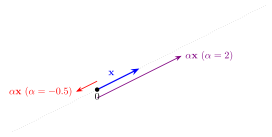
\includegraphics[width=0.8\textwidth]{images/escalar_vector}
    \caption{Efecto geométrico de la multiplicación escalar. Nótese cómo α=2 duplica la longitud, mientras que α=-0.5 reduce la longitud a la mitad e invierte el sentido.}
    \label{fig:escalar_vector}
\end{figure}

\subsubsection{Aplicaciones: Escalamiento y Control}

\begin{enumerate}
    \item \textbf{Agro (Proyección de Insumos):} 
    Suponga que el vector $\mathbf{d}$ representa la dosis de fertilizantes para \textbf{1 hectárea}: $\mathbf{d} = [100, 50, 30]^\top$ (kg de N, P, K).
    Si un agricultor desea fertilizar un lote de 15 hectáreas, el requerimiento total es simplemente el vector escalado por la superficie:

    \[ 
    \mathbf{Total} = 15 \cdot \mathbf{d} = \begin{pmatrix} 1500 \\ 750 \\ 450 \end{pmatrix} \text{ kg}. 
    \]
    
    \item \textbf{Mecatrónica (Ganancia de Control):}
    En un sistema de control de un robot, el  ``error'' de posición es un vector $\mathbf{e}$ (diferencia entre dónde está y dónde debería estar). El controlador aplica una corrección proporcional multiplicando ese error por una ganancia $K_p$ (un escalar).

    \[ 
    \mathbf{u} = K_p \cdot \mathbf{e} 
    \]

    Si $K_p$ es muy grande, el robot reacciona violentamente (gran vector de fuerza); si es pequeño, reacciona suavemente.
\end{enumerate}

\section{Producto punto (producto escalar)}

El \textbf{producto punto} es la operación fundamental para conectar la geometría (ángulos, longitudes) con el álgebra. Mide el grado de alineación entre dos vectores: si apuntan en la misma dirección, el valor es grande y positivo; si son perpendiculares, es cero; si apuntan en sentidos opuestos, es negativo.

\textbf{Definición formal.}

\[
\cdot : \mathbb{R}^n \times \mathbb{R}^n \to \mathbb{R}, \quad (\mathbf{x}, \mathbf{y}) \mapsto \mathbf{x} \cdot \mathbf{y} = \sum_{i=1}^{n} x_i y_i.
\]

\subsubsection{Interpretación Geométrica y Similitud}

Además de la operación algebraica componente a componente, el producto punto satisface una identidad geométrica fundamental, ilustrada en la Figura \ref{fig:producto_punto}:

\[
\mathbf{x} \cdot \mathbf{y} = \lVert \mathbf{x} \rVert \lVert \mathbf{y} \rVert \cos(\theta),
\]

donde $\theta$ es el ángulo entre los vectores. Esta relación permite aislar el término del coseno para definir la \textbf{Similitud Coseno}, una métrica esencial en Inteligencia Artificial para medir qué tan similares son dos vectores independientemente de su magnitud:

\begin{figure}[h]
    \centering
    \includegraphics[width=0.8\textwidth]{images/producto_punto}
    \caption{Relación entre magnitudes y ángulo. El producto punto conecta la longitud de los vectores con el coseno del ángulo θ que forman entre sí.}
    \label{fig:producto_punto}
\end{figure}

\[
\cos(\theta) = \frac{\mathbf{x} \cdot \mathbf{y}}{\lVert \mathbf{x} \rVert \lVert \mathbf{y} \rVert}.
\]

Como se observa en la Figura \ref{fig:producto_punto_geo}, geométricamente esto equivale a evaluar la proyección o "sombra" de un vector sobre el otro. Si el ángulo es cero (vectores alineados), la similitud es máxima (1); si son ortogonales (90°), es nula (0).



\begin{figure}[ht]
    \centering
    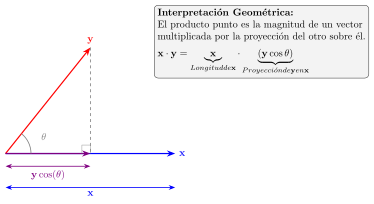
\includegraphics[width=0.8\textwidth]{images/producto_punto_cos}
    \caption{Interpretación de la proyección. La línea violeta muestra la componente de y que está ``alineada'' con x. El producto punto es el resultado de multiplicar esta proyección por la longitud total de x.}
    \label{fig:producto_punto_geo}
\end{figure}\paragraph{Aplicaciones en Ingeniería y Agro}

\begin{enumerate}
    \item \textbf{Agro (Firmas Espectrales):} 
    En teledetección, una planta sana tiene una ``firma''\ o vector ideal $\mathbf{v}_{sana}$ (valores de reflectancia en distintas bandas). Si el dron mide un vector actual $\mathbf{v}_{medido}$, calculamos el producto punto (normalizado) entre ambos.
    \begin{itemize}
        \item Si $\cos(\theta) \approx 1$, la firma es casi idéntica $\to$ Planta Sana.
        \item Si $\cos(\theta) \ll 1$, la alineación es baja $\to$ Posible estrés hídrico o plaga.
    \end{itemize}

    \item \textbf{Mecatrónica (Cálculo de Trabajo y Potencia):}
    Para un robot móvil, el trabajo mecánico $W$ realizado al mover una carga es el producto punto entre el vector de fuerza aplicada $\mathbf{F}$ y el vector de desplazamiento $\mathbf{d}$:

    \[ 
    W = \mathbf{F} \cdot \mathbf{d} = \lVert \mathbf{F} \rVert \lVert \mathbf{d} \rVert \cos(\theta) 
    \]

    Si el robot aplica fuerza perpendicular al movimiento ($\theta=90^\circ$), el producto punto es 0 y no se realiza trabajo útil (energía desperdiciada).

    \item \textbf{Administrativo (Sistemas de Puntuación):}
    Sea $\mathbf{w}$ un vector de ``pesos''\ o importancia para tres criterios (Costo, Calidad, Tiempo) y $\mathbf{x}$ el vector de puntajes de un proveedor. El puntaje total es simplemente:

    \[ 
    \text{Score} = \mathbf{w} \cdot \mathbf{x} = w_1 x_1 + w_2 x_2 + w_3 x_3 
    \]

    Esta es la base de las redes neuronales: una neurona realiza un producto punto entre los datos de entrada y sus pesos sinápticos.
\end{enumerate}

\subsubsection{Interpretación geométrica del Producto Punto}

El producto punto ($\mathbf{x} \cdot \mathbf{y}$) es mucho más que una suma de productos de componentes: es la operación geométrica fundamental que cuantifica cuánto dos vectores apuntan en la misma dirección. Esta noción de “alineación direccional” es la base de técnicas esenciales en inteligencia artificial, como la similitud coseno, la proyección ortogonal y el Análisis de Componentes Principales (PCA).

La definición geométrica del producto punto para dos vectores $\mathbf{x}, \mathbf{y} \in \mathbb{R}^n$ es:

\[
\mathbf{x} \cdot \mathbf{y} = \lVert \mathbf{x} \rVert \, \lVert \mathbf{y} \rVert \cos(\theta),
\]

donde $\lVert \mathbf{x} \rVert$ y $\lVert \mathbf{y} \rVert$ son las longitudes euclidianas de los vectores, y $\theta \in [0, \pi]$ es el ángulo entre ellos.

Esta fórmula revela tres casos clave:
\begin{itemize}
    \item Si $\theta = 0^\circ$ (vectores \textbf{paralelos y en la misma dirección}), $\cos(\theta) = 1$ y el producto punto es \textbf{máximo}.
    \item Si $\theta = 90^\circ$ (vectores \textbf{ortogonales}), $\cos(\theta) = 0$ y el producto punto es \textbf{cero}.
    \item Si $\theta = 180^\circ$ (vectores \textbf{opuestos}), $\cos(\theta) = -1$ y el producto punto es \textbf{mínimo} (negativo).
\end{itemize}

\textbf{Conexión con aplicaciones en IA y agro-ambiente.}  
En el análisis de datos, el producto punto permite:
\begin{itemize}
    \item Comparar perfiles de fertilización entre parcelas: si $\theta$ es pequeño, las prácticas son similares.
    \item Detectar animales atípicos en un hato: un vector fisiológico con $\theta$ grande respecto a la media indica una posible anomalía.
    \item Calcular la similitud coseno (normalizando las magnitudes): $\frac{\mathbf{x} \cdot \mathbf{y}}{\lVert \mathbf{x} \rVert \lVert \mathbf{y} \rVert} = \cos(\theta)$, que mide \textit{solo} la alineación, ignorando la escala.
\end{itemize}

Esta interpretación geométrica es el primer paso hacia la comprensión de cómo los algoritmos de IA ``ven'' y comparan datos en espacios multidimensionales.
\paragraph{Dependencia de la Proyección}
El concepto más fundamental es la relación con la proyección ortogonal, como se ilustra en la figura \ref{fig:producto_punto_geo}. El término $\lVert \mathbf{y} \rVert \cos(\theta)$ representa precisamente la longitud de la \textit{componente} del vector $\mathbf{y}$ que está alineada con $\mathbf{x}$ (la proyección, $\mathrm{proj}_{\mathbf{x}} \mathbf{y}$).

Por lo tanto, el producto punto puede reescribirse como:

\[
\mathbf{x} \cdot \mathbf{y} = \lVert \mathbf{x} \rVert \cdot \left( \lVert \mathbf{y} \rVert \cos(\theta) \right) = \lVert \mathbf{x} \rVert \cdot \lVert \mathrm{proj}_{\mathbf{x}} \mathbf{y} \rVert.
\]

El producto punto es, en esencia, la magnitud de $\mathbf{x}$ multiplicada por la longitud de la ``sombra'' que $\mathbf{y}$ proyecta sobre $\mathbf{x}$. El signo de $\mathbf{x} \cdot \mathbf{y}$ depende únicamente del $\cos(\theta)$.

\paragraph{Casos Críticos}
El valor del producto punto está dominado por el coseno del ángulo $\theta$, asumiendo que las magnitudes de los vectores son positivas:

\begin{enumerate}
    \item \textbf{Alineación Perfecta ($\theta = 0^\circ$):}
    Si $\mathbf{x}$ y $\mathbf{y}$ apuntan exactamente en la misma dirección, $\cos(0^\circ) = 1$.
    
    \[
    \mathbf{x} \cdot \mathbf{y} = \lVert \mathbf{x} \rVert \lVert \mathbf{y} \rVert.
    \]

    El producto punto es \textit{máximo y positivo}. En IA, esto indica máxima similitud o máxima compatibilidad direccional.

    \item \textbf{Ortogonalidad ($\theta = 90^\circ$):}
    Si $\mathbf{x}$ y $\mathbf{y}$ son perpendiculares (ortogonales), $\cos(90^\circ) = 0$.

    \[
    \mathbf{x} \cdot \mathbf{y} = 0.
    \]

    El producto punto es \textit{cero}, indicando que los vectores no tienen ninguna componente en común y son linealmente independientes, un principio clave en la decorrelación de datos (ej. PCA).

    \item \textbf{Alineación Opuesta ($\theta = 180^\circ$):}
    Si $\mathbf{x}$ y $\mathbf{y}$ apuntan en direcciones opuestas, $\cos(180^\circ) = -1$.

    \[
    \mathbf{x} \cdot \mathbf{y} = -\lVert \mathbf{x} \rVert \lVert \mathbf{y} \rVert.
    \]

    El producto punto es \textit{mínimo y negativo}, indicando la máxima disimilitud o incompatibilidad.
\end{enumerate}
    

% \begin{figure}[ht]
% \centering
% \begin{tikzpicture}[scale=1.4]

%     % Origen
%     \coordinate (O) at (0,0);
%     \coordinate (X) at (3.5, 1.5);
%     \coordinate (Y) at (1.0, 3.5);

%     % Cálculo del ángulo entre X y Y
%     \pgfmathsetmacro{\angleX}{atan2(1.5, 3.5)} % ángulo de x respecto al eje x1
%     \pgfmathsetmacro{\angleY}{atan2(3.5, 1.0)} % ángulo de y respecto al eje x1
%     \pgfmathsetmacro{\angleTheta}{\angleY - \angleX}

%     % Ejes
%     \draw[->, gray!50] (-0.5,0) -- (4,0) node[right] {$x_1$};
%     \draw[->, gray!50] (0,-0.5) -- (0,4) node[above] {$x_2$};

%     % Vectores
%     \draw[->, blue, very thick] (O) -- (X)
%         node[midway, below right] {$\mathbf{x}$};
%     \draw[->, red, very thick] (O) -- (Y)
%         node[midway, above left] {$\mathbf{y}$};

%     % Proyección de y sobre x
%     \pgfmathsetmacro{\scale}{
%         ((3.5)*(1.0) + (1.5)*(3.5)) /
%         ((3.5)*(3.5) + (1.5)*(1.5))
%     }
%     \coordinate (P) at ({\scale*3.5}, {\scale*1.5});
%     \draw[dashed, red!70] (Y) -- (P);
%     \draw[->, red!70, thick] (O) -- (P)
%         node[midway, below] {$\mathrm{proj}_{\mathbf{x}} \mathbf{y}$};

%     % Ángulo theta CON FLECHAS EN AMBOS EXTREMOS
%     \draw[
%         purple,
%         thick,
%         ->
%     ]
%     (O) ++({\angleX}:1.0)
%     arc[
%         start angle=\angleX,
%         end angle=\angleY,
%         radius=1.0
%     ];

%     \node[purple] at ({\angleX + 0.5*\angleTheta}:1.3) {$\theta$};

% \end{tikzpicture}
% \caption{Interpretación geométrica del producto punto. El ángulo $\theta$ está dibujado entre los vectores $\mathbf{x}$ e $\mathbf{y}$. El producto punto es proporcional a la magnitud de la proyección de $\mathbf{y}$ sobre $\mathbf{x}$.}
% \label{fig:producto_punto_geometrico_corregido}
% \end{figure}

\subsubsection{Síntesis y Aplicaciones Contextuales del Producto Punto}

La utilidad del producto punto ($\mathbf{x} \cdot \mathbf{y}$) radica en su capacidad para actuar como una medida de \textit{alineación multidimensional} o \textit{similitud} entre vectores. Su valor es grande cuando las magnitudes y la alineación son altas, reflejando perfiles compatibles. Este concepto es la base de la \textbf{similitud coseno} ($\cos(\theta) = \frac{\mathbf{x} \cdot \mathbf{y}}{\lVert \mathbf{x} \rVert \lVert \mathbf{y} \rVert}$), ampliamente usada en motores de recomendación y clustering.

\vspace{0.3cm}

\paragraph{Ejemplos en Contextos de Modelado Híbrido (Agronómico y Zootécnico)}

\begin{itemize}
    \item \textbf{Ejemplo Agronómico.}
    Considere dos parcelas de maíz caracterizadas por el vector de insumos aplicados:

    \[
    \mathbf{x} = \begin{pmatrix} 120 \\ 50 \\ 3 \end{pmatrix} \text{ (kg/ha de N, P, K)}, \quad
    \mathbf{y} = \begin{pmatrix} 100 \\ 60 \\ 4 \end{pmatrix}.
    \]

    El producto punto $\mathbf{x} \cdot \mathbf{y} = 12\,000 + 3\,000 + 12 = 15\,012$ es alto, lo que sugiere un perfil de fertilización similar. Esta medida agrupa parcelas con prácticas comparables.

    \item \textbf{Ejemplo Zootécnico.}
    Considere dos vacas lecheras descritas por su historial productivo en una ventana de control:

    \[
    \mathbf{x} = \begin{pmatrix} 28 \\ 4{,}2 \\ 38 \end{pmatrix}, \quad
    \mathbf{y} = \begin{pmatrix} 30 \\ 4{,}0 \\ 39 \end{pmatrix},
    \]

    donde las componentes representan días en lactancia, producción diaria (L/día) y contenido de grasa (\%).
    El producto punto:

    \[
    \mathbf{x} \cdot \mathbf{y} = (28)(30) + (4{,}2)(4{,}0) + (38)(39) = 2338{,}8.
    \]

    Este valor alto refleja perfiles productivos similares: producción alta, lactancia avanzada y elevado contenido de grasa. Esta medida es útil en sistemas de segmentación de hatos.
\end{itemize}

\vspace{0.3cm}

\textbf{Otros Contextos Aplicados}

\begin{itemize}
    \item \textbf{Ambiental:} Dos estaciones de monitoreo registran concentraciones medias (en $\mathrm{\mu g/m^3}$) de $\mathrm{PM_{2.5}}$, $\mathrm{NO_2}$ y $\mathrm{O_3}$: $\mathbf{a}$ y $\mathbf{b}$. Un producto punto alto sugiere un patrón similar de contaminación, útil para agrupar zonas con fuentes emisoras comunes.

    \item \textbf{Administrativo:} Dos propuestas presupuestales $\mathbf{p}$ y $\mathbf{q}$ (para rubros como infraestructura, capacitación, operación) tienen un producto punto que cuantifica la \textit{alineación de prioridades presupuestales}.

    \item \textbf{Diseño (Industrial/Agrícola):} Dos prototipos de invernadero $\mathbf{d}_1$ y $\mathbf{d}_2$ (descritos por área, sensores, consumo energético). Un producto punto elevado indica diseños estructuralmente similares, facilitando la clasificación de alternativas.
\end{itemize}

En resumen, el producto punto sirve como un indicador fundamental de cuán coherentes o compatibles son dos conjuntos de mediciones o características multidimensionales.
\section{Laboratorio de Programación: Aritmética Tensorial en la Práctica}

En esta sección, trasladamos las operaciones de suma, escalamiento y producto punto al código. En IA, estas operaciones no se realizan mediante bucles (\textit{for loops}), sino a través de \textbf{operaciones vectorizadas}, las cuales aprovechan el paralelismo del procesador.

\subsection{Implementación de Suma y Escalamiento}

La suma de vectores requiere que ambos tengan la misma dimensión (\textit{shape}). La multiplicación por un escalar, en cambio, utiliza un mecanismo llamado \textbf{Broadcasting}, donde el escalar se ``difunde'' sobre todos los elementos del vector.

\begin{lstlisting}[language=Python, caption=Suma de vectores y multiplicación por escalar]
import numpy as np
import torch

# 1. Suma de vectores (Agro: Integración de dosis de fertilizante)
dosis_neta = np.array([50, 20, 10])  # N, P, K inicial
suplemento = np.array([10,  5,  5])  # Refuerzo aplicado
dosis_total = dosis_neta + suplemento
print(f''Dosis Total (Vector): {dosis_total}'')

# 2. Multiplicación por Escalar (Mecatrónica: Control de Ganancia)
# Escalar una señal de sensor de torque
torque_raw = torch.tensor([1.2, 0.8, 1.5])
ganancia = 2.5
torque_ajustado = ganancia * torque_raw
print(f''Torque ajustado: {torque_ajustado}'')
\end{lstlisting}

\subsection{El Producto Punto: Cuantificando la Afinidad}

El producto punto es la operación más importante en IA. En Python, podemos ejecutarlo usando el operador \texttt{@} (recomendado en versiones modernas) o las funciones específicas de las librerías.

\begin{lstlisting}[language=Python, caption=Cálculo del Producto Punto]
# Vectores de ejemplo (Administración: Gastos vs Presupuesto)
unidades = np.array([10, 5, 20])   # Cantidad de productos comprados
precios = np.array([1.5, 10.0, 0.5]) # Precio unitario por categoría

# Producto punto: Suma de (unidades[i] * precios[i])
gasto_total = np.dot(unidades, precios)
# Forma alternativa (estándar en álgebra lineal de Python):
gasto_total_alt = unidades @ precios

print(f''Gasto total calculado via producto punto: ${gasto_total}'')
\end{lstlisting}


\subsection{Aplicaciones Sectoriales en Código}

\begin{quote}{Mecatrónica: Resultante de Fuerzas}
    En un brazo robótico, si dos motores ejercen fuerzas representadas por los vectores $\mathbf{f}_1$ y $\mathbf{f}_2$, la fuerza resultante sobre el efector final es simplemente \texttt{$f_res = f1 + f2$}. La magnitud de esta fuerza se obtiene con \texttt{np.linalg.norm($f_res$)}.
\end{quote}

\begin{quote}{Agroindustrial: Mezclas y Diluciones}
    Si un vector $\mathbf{v}$ representa la concentración de azúcares y acidez de un lote de jugo, y queremos diluirlo al $50\%$, aplicamos \texttt{$nuevo_lote = 0.5 * v$}. El producto punto se usa para calcular el costo total de la mezcla si tenemos un vector de precios por litro de cada componente.
\end{quote}

\subsection*{Resumen de Funciones Clave}

\begin{table}[ht]
\centering
\begin{tabular}{|l|l|l|}
\hline
\textbf{Operación} & \textbf{Sintaxis NumPy} & \textbf{Sintaxis PyTorch} \\ \hline
Suma               & \texttt{a + b}          & \texttt{a + b}            \\ \hline
Escalamiento       & \texttt{k * a}          & \texttt{k * a}            \\ \hline
Producto Punto     & \texttt{np.dot(a, b)}   & \texttt{torch.dot(a, b)}  \\ \hline
Producto de Matriz & \texttt{a @ b}          & \texttt{torch.matmul(a, b)} \\ \hline
\end{tabular}
\caption{Comparativa de funciones para aritmética tensorial.}
\end{table}
\section{Multiplicación Matriz-Vector: El Motor de las Redes Neuronales}

Antes de entrar en el formalismo, entendamos la intuición: si un vector representa un dato (ej. una parcela, un animal, una propuesta), multiplicar ese vector por una matriz es equivalente a procesar ese dato a través de un banco de filtros. La matriz toma la información cruda, mezcla sus componentes según ciertas reglas (pesos) y produce una nueva representación más útil para la toma de decisiones.

Esta operación es el corazón de las redes neuronales profundas (Deep Learning).

\paragraph{Definición formal}
Sea $\mathbf{W} \in \mathbb{R}^{m \times n}$ una matriz y $\mathbf{x} \in \mathbb{R}^n$ un vector de entrada. Su producto es un nuevo vector $\mathbf{z} \in \mathbb{R}^m$ definido por:

\[
\mathbf{z} = \mathbf{W} \mathbf{x} =
\begin{pmatrix}
\mathbf{fila}_1(\mathbf{W}) \cdot \mathbf{x} \\
\vdots \\
\mathbf{fila}_m(\mathbf{W}) \cdot \mathbf{x}
\end{pmatrix}.
\]

Cada entrada $z_i$ es el \textbf{producto punto} entre la fila $i$-ésima de la matriz y el vector $\mathbf{x}$. Para que la operación sea válida, el número de columnas de la matriz ($n$) debe coincidir con la dimensión de entrada del vector.

\paragraph{Ejemplo Teórico: Transformación de Insumos a Nutrientes}

Imaginemos un sistema inteligente para la formulación de raciones en ganado lechero. Queremos calcular el aporte nutricional total a partir de una mezcla de ingredientes.

\textbf{1. El Vector de Entrada ($\mathbf{x}$):}
Representa la cantidad de materia prima (en kg) que vamos a utilizar en la mezcla.

\[
\mathbf{x} = \begin{pmatrix} 10 \\ 5 \end{pmatrix}
\begin{matrix} \text{(kg de Maíz)} \\ \text{(kg de Soya)} \end{matrix}
\]

Aquí, $n=2$ (tenemos 2 ingredientes).

\textbf{2. La Matriz de Pesos ($\mathbf{W}$):}
Representa el contenido nutricional por cada kg de ingrediente.
\begin{itemize}
    \item La \textbf{Fila 1} corresponde a la \textbf{Proteína Cruda} (en kg/kg).
    \item La \textbf{Fila 2} corresponde a la \textbf{Energía Neta} (en Mcal/kg).
\end{itemize}

\[
\mathbf{W} = 
\begin{pmatrix} 
0{,}08 & 0{,}45 \\ 
3{,}20 & 2{,}80 
\end{pmatrix}
\begin{matrix} \leftarrow \text{Perfil de Proteína} \\ \leftarrow \text{Perfil de Energía} \end{matrix}
\]

Aquí, $m=2$ (tenemos 2 métricas de salida). Note que las columnas ($n=2$) coinciden con los ingredientes (Maíz y Soya).

\textbf{3. El Cálculo ($\mathbf{z} = \mathbf{W}\mathbf{x}$):}
Aplicamos la definición del producto punto fila por columna:

\[
\mathbf{z} = 
\begin{pmatrix}
(\text{Fila}_1 \cdot \mathbf{x}) \\
(\text{Fila}_2 \cdot \mathbf{x})
\end{pmatrix}
=
\begin{pmatrix}
(0{,}08)(10) + (0{,}45)(5) \\
(3{,}20)(10) + (2{,}80)(5)
\end{pmatrix}
\]

\[
\mathbf{z} = 
\begin{pmatrix}
0{,}8 + 2{,}25 \\
32{,}0 + 14{,}0
\end{pmatrix}
=
\begin{pmatrix}
3{,}05 \\
46{,}0
\end{pmatrix}
\begin{matrix} \text{kg de Proteína Total} \\ \text{Mcal de Energía Total} \end{matrix}
\]

\textbf{Interpretación en Inteligencia Artificial:}
En este ejemplo, la matriz $\mathbf{W}$ codifica el ``conocimiento'' del sistema sobre los alimentos.
\begin{itemize}
    \item En una Red Neuronal, $\mathbf{x}$ serían los datos de entrada, $\mathbf{W}$ serían los \textit{pesos sinápticos} aprendidos durante el entrenamiento, y $\mathbf{z}$ sería la activación resultante.
    \item La operación $\mathbf{W}\mathbf{x}$ transforma el espacio de ``kilos de comida'' al espacio de ``requerimientos nutricionales''.
\end{itemize}

\paragraph{Enfoque en Redes Neuronales: La Capa Densa}

En el contexto de la inteligencia artificial, esta operación no es solo álgebra; es la definición de una \textbf{capa densa} (fully connected layer). La ecuación fundamental que ejecuta una neurona artificial (antes de la activación no lineal) es:

\[
\mathbf{z} = \mathbf{W} \mathbf{x} + \mathbf{b},
\]

donde cada elemento cumple un rol biológico-computacional preciso:

\begin{itemize}
    \item $\mathbf{x}$ (Entradas): Son las señales recibidas (ej. variables del cultivo o píxeles de una imagen).
    \item $\mathbf{W}$ (Matriz de Pesos): Es la ``memoria'' del modelo. Cada fila de $\mathbf{W}$ representa una neurona, y sus valores indican qué tanto importa cada entrada para esa neurona específica.
    \item $\mathbf{z}$ (Activaciones): Es la respuesta de las neuronas ante el estímulo $\mathbf{x}$.
\end{itemize}

\paragraph{Ejemplo aplicado: Neuronas ``Expertas'' en Evaluación Administrativa}

Imagine que una IA administrativa debe evaluar automáticamente propuestas de proyectos. El vector de entrada $\mathbf{x}$ contiene $n=4$ variables presupuestales: $(\text{infraestructura}, \text{capacitación}, \text{operación}, \text{monitoreo})$.

La red neuronal tiene una capa con $m=2$ neuronas, donde cada una se ha especializado (aprendido) para detectar un criterio diferente:
\begin{enumerate}
    \item \textbf{Neurona 1:} Evalúa el ``Equilibrio Estratégico''.
    \item \textbf{Neurona 2:} Evalúa la ``Sostenibilidad Ambiental''.
\end{enumerate}

La matriz de pesos $\mathbf{W} \in \mathbb{R}^{2 \times 4}$ codifica estas prioridades:

\[
\mathbf{W} =
\begin{pmatrix}
0{,}3 & 0{,}3 & 0{,}3 & 0{,}1 \\  % Neurona 1: Pondera todo por igual (busca equilibrio)
0{,}1 & 0{,}2 & 0{,}4 & 0{,}3      % Neurona 2: Prioriza operación y monitoreo (sostenibilidad)
\end{pmatrix}.
\]

Si llega una propuesta con el siguiente perfil de inversión (en millones):

\[
\mathbf{x} = (300, 80, 220, 75)^\top.
\]

El paso hacia adelante (\textit{forward pass}) de la red calcula:

\[
\mathbf{z} = \mathbf{W} \mathbf{x} =
\begin{pmatrix}
(0{,}3)(300) + (0{,}3)(80) + (0{,}3)(220) + (0{,}1)(75) \\
(0{,}1)(300) + (0{,}2)(80) + (0{,}4)(220) + (0{,}3)(75)
\end{pmatrix}
=
\begin{pmatrix}
187{,}5 \\
156{,}5
\end{pmatrix}.
\]

\textbf{Interpretación del resultado:}
El vector de salida $\mathbf{z}$ nos dice que esta propuesta tiene una puntuación alta en equilibrio ($187{,}5$) y moderada en sostenibilidad ($156{,}5$).

\paragraph{Por qué esto es fundamental}
Este mecanismo permite que una red neuronal transforme datos brutos en conceptos abstractos. En este ejemplo, pasamos de ``dinero en rubros'' (espacio de entrada $\mathbb{R}^4$) a ``calidad estratégica'' (espacio de características $\mathbb{R}^2$). Durante el entrenamiento, el algoritmo de \textit{backpropagation} ajusta los valores de la matriz $\mathbf{W}$ para minimizar el error en la evaluación, ``aprendiendo'' así los pesos ideales para clasificar proyectos correctamente.

\section{Producto de Matrices}

Las matrices constituyen la estructura algebraica fundamental para representar datos tabulares, transformaciones lineales y relaciones entre variables en el contexto de la Inteligencia Artificial. A continuación, se detallan las operaciones y propiedades esenciales para el modelado de datos.

La multiplicación de matrices actúa como el motor computacional del aprendizaje profundo. Esta operación no solo generaliza el producto punto, sino que permite ejecutar múltiples operaciones simultáneamente (lo que conocemos como procesamiento en lote o \textit{batch}) y realizar la composición de transformaciones lineales.

\subsubsection{Regla de Dimensiones}
Para que el producto matricial $\mathbf{A}\mathbf{B}$ esté definido, las dimensiones internas deben coincidir (es decir, el número de columnas de la primera debe igualar al número de filas de la segunda):

\[
\underbrace{\mathbf{A}}_{m \times \mathbf{n}} \quad \times \quad \underbrace{\mathbf{B}}_{\mathbf{n} \times p} \quad = \quad \underbrace{\mathbf{C}}_{m \times p}
\]

\paragraph{Definición Formal}
Dadas $\mathbf{A} \in \mathbb{R}^{m \times n}$ y $\mathbf{B} \in \mathbb{R}^{n \times p}$, su producto $\mathbf{C} = \mathbf{A}\mathbf{B} \in \mathbb{R}^{m \times p}$ se define entrada por entrada. Como se ilustra conceptualmente en la Figura \ref{fig:mult_matrices}, el valor $c_{ij}$ se obtiene mediante el producto punto entre la fila $i$ de $\mathbf{A}$ y la columna $j$ de $\mathbf{B}$:

\[
c_{ij} = \mathbf{fila}_i(\mathbf{A}) \cdot \mathbf{columna}_j(\mathbf{B}) = \sum_{k=1}^{n} a_{ik} b_{kj}.
\]

\begin{figure}[ht]
    \centering
    \includegraphics[width=0.8\linewidth]{images/producto_matriz_vector}
    \caption{Visualización del producto matricial. El elemento resultante $c_{ij}$ captura la interacción total entre la fila $i$ de la matriz izquierda y la columna $j$ de la matriz derecha.}
    \label{fig:mult_matrices}
\end{figure}
\textbf{Propiedades clave:}
\begin{itemize}
    \item \textbf{No Conmutatividad:} En general, $\mathbf{A}\mathbf{B} \neq \mathbf{B}\mathbf{A}$. El orden importa: rotar y luego trasladar no es lo mismo que trasladar y luego rotar.
    \item \textbf{Asociatividad:} $(\mathbf{A}\mathbf{B})\mathbf{C} = \mathbf{A}(\mathbf{B}\mathbf{C})$. Esto es vital en Deep Learning para optimizar el cómputo en capas profundas.
\end{itemize}

\begin{quote}{Ejemplo Práctico: Lotes $\times$ Proveedores}
Imaginemos que queremos calcular costos para diferentes escenarios.
\begin{itemize}
    \item $\mathbf{A}$ (Requerimientos): 2 Lotes (filas) necesitan cantidades de 3 insumos (columnas: N, P, K).
    \item $\mathbf{B}$ (Precios): Esos 3 insumos tienen precios diferentes en 2 Proveedores distintos (columnas).
\end{itemize}

\[
\mathbf{A}_{(2 \times 3)} = 
\begin{pmatrix} 
10 & 20 & 5 \\ 
15 & 10 & 2 
\end{pmatrix}, \quad
\mathbf{B}_{(3 \times 2)} = 
\begin{pmatrix} 
2 & 3 \\ 
4 & 4 \\ 
10 & 8 
\end{pmatrix}
\]

El producto $\mathbf{C} = \mathbf{AB}$ nos dará una matriz de $2 \times 2$ donde cada elemento $c_{ij}$ es el \textbf{costo total} del Lote $i$ comprando al Proveedor $j$.

Realizamos los cálculos para cada celda:
\begin{align*}
c_{11} &= (10\cdot 2) + (20 \cdot 4) + (5 \cdot 10) = 20 + 80 + 50 = 150 \\
c_{12} &= (10\cdot 3) + (20 \cdot 4) + (5 \cdot 8) = 30 + 80 + 40 = 150 \\
c_{21} &= (15\cdot 2) + (10 \cdot 4) + (2 \cdot 10) = 30 + 40 + 20 = 90 \\
c_{22} &= (15\cdot 3) + (10 \cdot 4) + (2 \cdot 8) = 45 + 40 + 16 = 101
\end{align*}

El resultado final es:

\[
\mathbf{C} = 
\begin{pmatrix} 
150 & 150 \\ 
90 & 101 
\end{pmatrix}
\]

\textbf{Interpretación para toma de decisiones:}
\begin{itemize}
    \item Para el \textbf{Lote 1} (Fila 1), ambos proveedores resultan en el mismo costo total (\$150), aunque los precios unitarios sean distintos.
    \item Para el \textbf{Lote 2} (Fila 2), es más económico comprar al \textbf{Proveedor 1} (\$90) que al Proveedor 2 (\$101).
\end{itemize}
Esta operación permite evaluar múltiples escenarios económicos de forma simultánea.
\end{quote}
\section{Escalares asociados: Traza, Determinante y Rango}

Antes de analizar propiedades más complejas, definimos tres escalares que resumen la estructura de una matriz cuadrada $\mathbf{A} \in \mathbb{R}^{n \times n}$:

\begin{itemize}
    \item \textbf{Traza ($\mathrm{tr}$):} La suma de los elementos de la diagonal principal. En matrices de covarianza, representa la \textit{varianza total} del sistema.
    \item \textbf{Determinante ($\det$):} Una medida del cambio de volumen que produce la matriz como transformación lineal. Si $\det(\mathbf{A}) = 0$, la matriz ``aplasta'' el espacio y destruye información.
    \item \textbf{Rango:} El número máximo de filas o columnas linealmente independientes. Indica la cantidad de información no redundante en los datos.
\end{itemize}

\paragraph{El Determinante}

El \textbf{determinante} es una función escalar que asigna a cada matriz cuadrada $\mathbf{A} \in \mathbb{R}^{n \times n}$ un número real, denotado como $\det(\mathbf{A})$ o $|\mathbf{A}|$. Este valor condensa información crítica sobre la naturaleza geométrica y algebraica de la matriz.



\paragraph{Interpretación geométrica}
En el contexto del análisis de datos, el determinante representa el \textbf{factor de escala} del volumen (o área en 2D) cuando la matriz $\mathbf{A}$ actúa como una transformación lineal.
\begin{itemize}
    \item Si $|\det(\mathbf{A})| > 1$, la transformación expande el espacio.
    \item Si $0 < |\det(\mathbf{A})| < 1$, la transformación contrae el espacio.
    \item Si $\det(\mathbf{A}) = 0$, la transformación ``aplasta'' el volumen hasta convertirlo en una superficie, línea o punto (pérdida de dimensionalidad).
\end{itemize}

\paragraph{Cálculo en $2 \times 2$}
Para una matriz de $\mathbb{R}^{2 \times 2}$, la fórmula es:

\[
\begin{vmatrix} 
a & b \\ 
c & d 
\end{vmatrix} = ad - bc
\]

\paragraph{Singularidad e Invertibilidad}
La propiedad más importante para la inteligencia artificial es su relación con la inversión de matrices:

\[
\mathbf{A} \text{ es invertible} \iff \det(\mathbf{A}) \neq 0.
\]

Una matriz con determinante cero se llama \textbf{singular}. En términos de datos, esto implica que las filas (o columnas) son linealmente dependientes, es decir, existe redundancia perfecta en la información (colinealidad).

\paragraph{Ejemplo Agro-Ambiental: Detección de Redundancia}
Suponga que intentamos modelar el crecimiento de un cultivo usando dos variables que creemos distintas: $x_1$ (agua de riego en L) y $x_2$ (tiempo de riego en minutos). Sin embargo, si el sistema de riego tiene un flujo constante, $x_1$ es exactamente proporcional a $x_2$.

La matriz de correlación o covarianza de estos datos tendría la forma:

\[
\mathbf{C} = 
\begin{pmatrix} 
1 & 1 \\ 
1 & 1 
\end{pmatrix}.
\]

Calculando el determinante:

\[
\det(\mathbf{C}) = (1)(1) - (1)(1) = 0.
\]

El determinante nulo nos alerta matemáticamente de que no tenemos dos dimensiones reales de información, sino solo una. Intentar invertir esta matriz para un modelo de regresión lineal generará un error computacional, indicando que debemos eliminar una de las variables redundantes antes de entrenar el modelo.


\section{Inversa de una matriz}

La \textbf{inversa} de una matriz cuadrada $\mathbf{A} \in \mathbb{R}^{n \times n}$, denotada $\mathbf{A}^{-1}$, es la matriz única que satisface:

\[
\mathbf{A} \mathbf{A}^{-1} = \mathbf{A}^{-1} \mathbf{A} = \mathbf{I}_n,
\]

donde $\mathbf{I}_n$ es la matriz identidad (con 1s en la diagonal y 0s fuera).

\paragraph{Condición de existencia}
Una matriz $\mathbf{A}$ es invertible (o no singular) si y solo si cumple cualquiera de estas condiciones equivalentes:
\begin{itemize}
    \item $\det(\mathbf{A}) \neq 0$,
    \item Su rango es completo ($\mathrm{rango}(\mathbf{A}) = n$),
    \item Sus columnas son linealmente independientes (no hay redundancia perfecta entre variables).
\end{itemize}

\paragraph{Relevancia en IA}
\begin{itemize}
    \item \textbf{Regresión Lineal:} Los coeficientes óptimos se estiman como $\boldsymbol{\beta} = (\mathbf{X}^\top \mathbf{X})^{-1} \mathbf{X}^\top \mathbf{y}$.
    \item \textbf{Distancia de Mahalanobis:} $\sqrt{(\mathbf{x}-\boldsymbol{\mu})^\top \mathbf{\Sigma}^{-1} (\mathbf{x}-\boldsymbol{\mu})}$. Usada para detectar outliers multivariados (ej. animales enfermos con patrones fisiológicos atípicos).
\end{itemize}

\textbf{Ejemplo agronómico.} Para predecir rendimiento ($y$) a partir de N y P ($\mathbf{X}$), necesitamos calcular $(\mathbf{X}^\top \mathbf{X})^{-1}$. Si

\[
\mathbf{X}^\top \mathbf{X} = \begin{pmatrix} 5 & 2 \\ 2 & 2 \end{pmatrix} \implies \det = 10 - 4 = 6 \neq 0.
\]

Como el determinante es no nulo, la inversa existe y el modelo tiene solución única:

\[
(\mathbf{X}^\top \mathbf{X})^{-1} = \frac{1}{6} \begin{pmatrix} 2 & -2 \\ -2 & 5 \end{pmatrix}.
\]


\section{Implementación en Python: Operaciones Matriciales}

En el ecosistema de Python científico (NumPy), las operaciones matriciales están altamente optimizadas. A diferencia de otros lenguajes donde se requieren bucles, aquí operamos directamente sobre las estructuras de datos.

\subsection{El Operador Producto (@)}
Desde Python 3.5, el estándar para la multiplicación de matrices es el operador arroba (\texttt{@}). Este operador verifica automáticamente la consistencia de las dimensiones internas.

\subsection{Álgebra Lineal con \texttt{numpy.linalg}}
Para operaciones más avanzadas como determinantes, trazas e inversas, utilizamos el submódulo de álgebra lineal. A continuación, se presenta una implementación completa.

% Usamos lstlisting. El script se encargará de colorearlo.
\begin{lstlisting}[language=Python, caption=Operaciones matriciales en NumPy]
import numpy as np

# --- 1. PRODUCTO MATRICIAL (@) ---
# Matriz A (2x3) y B (3x2)
A = np.array([[10, 20, 5], 
              [15, 10, 2]])
B = np.array([[2, 3], 
              [4, 4], 
              [10, 8]])

# Producto punto generalizado
C = A @ B
print(f"Producto C (2x2):\n{C}\n")

# --- 2. PROPIEDADES ---
# Ejemplo A: Matriz 2x2
M_2x2 = np.array([[4, 1],
                  [2, 3]])

# Traza (suma diagonal) y Determinante
traza_2 = np.trace(M_2x2)       
det_2   = np.linalg.det(M_2x2)  

print(f"Matriz 2x2 -> Traza: {traza_2}, Det: {det_2:.2f}")

# --- 3. INVERSA Y VERIFICACIÓN ---
M_3x3 = np.array([[1, 0, 2], [0, 3, 1], [2, 1, 0]])
det_3 = np.linalg.det(M_3x3)

if det_3 != 0:
    M_inv = np.linalg.inv(M_3x3)
    
    # VERIFICACIÓN: A @ A_inv = Identidad
    # Usamos allclose por precisión flotante
    identidad_calc = M_3x3 @ M_inv
    es_identidad = np.allclose(identidad_calc, np.eye(3))
    
    print(f"¿Es Identidad? {es_identidad}")
else:
    print("Matriz singular.")
\end{lstlisting}

% Usamos alertblock. El script lo convertirá en una nota visual.
\begin{alertblock}{Nota sobre Punto Flotante}
Al calcular la inversa, es común obtener números como \texttt{0.9999999} en lugar de \texttt{1.0} debido a la precisión finita de las computadoras. Por eso, en lugar de comparar con \texttt{==}, utilizamos \texttt{np.allclose()} para verificar si el resultado es matemáticamente correcto dentro de una tolerancia aceptable.
\end{alertblock}

\subsubsection{Errores comunes y buenas prácticas}

\begin{enumerate}
    \item \textbf{El operador correcto:} 
    No confunda el operador \texttt{@} con el asterisco \texttt{*}. 
    \begin{itemize}
        \item \texttt{A @ B}: Producto matricial (fila por columna).
        \item \texttt{A * B}: Producto elemento a elemento (requiere mismas dimensiones exactas o broadcasting).
    \end{itemize}
    
    \item \textbf{Gestión de dimensiones:}
    Si intenta multiplicar matrices incompatibles, NumPy arrojará un error. Es vital verificar siempre \texttt{.shape}.
    
\begin{lstlisting}[language=Python]
# Intentar multiplicar A por sí misma: (2x3) @ (2x3)
try:
    Error = A @ A 
except ValueError as e:
    print(''Error de dimensión:'', e)
    
# Salida:
# ValueError: matmul: Input operand 1 has a mismatch in its core dimension 0...
# (size 3 is different from 2)
\end{lstlisting}
\end{enumerate}

\begin{tcolorbox}[colback=blue!5, colframe=blue!40, title=Nota de Ingeniería]
En el código de redes neuronales (como TensorFlow o PyTorch), la operación \texttt{capa\_oculta @ pesos} ocurre millones de veces por segundo. La eficiencia de esta operación es la razón por la que usamos GPUs (Tarjetas Gráficas), ya que están diseñadas por hardware para realizar multiplicaciones de matrices en paralelo masivo.
\end{tcolorbox}



\section{Operaciones con Tensores en Bioingeniería}

A diferencia de las matrices, donde el producto punto es la estrella, en los tensores operamos frecuentemente con \textbf{filtrado (convolución)}, \textbf{operaciones elemento a elemento} (Hadamard) y \textbf{re-dimensionamiento} (Reshaping).

\begin{quote}{Caso de Estudio: Detección de Tumores en MRI}
Una Resonancia Magnética (MRI) del cerebro no es una foto plana; es una volumetría.
Podemos representarla como un tensor $\mathcal{X}$ de dimensiones $256 \times 256 \times 120$:
\begin{itemize}
    \item $256 \times 256$: Resolución de cada ``rebanada'' (slice) de imagen (alto $\times$ ancho).
    \item $120$: El número de rebanadas tomadas desde la base del cráneo hasta la coronilla (profundidad).
\end{itemize}

\textbf{Operación 1: Aplicación de una Máscara (Producto Hadamard)}
Para aislar el cerebro y eliminar el cráneo o el fondo, multiplicamos el tensor de la imagen $\mathcal{X}$ por un tensor binario ``máscara'' $\mathcal{M}$ (donde 1 es tejido cerebral y 0 es hueso/fondo).

\[
\mathcal{Y} = \mathcal{X} \odot \mathcal{M} \quad \implies \quad y_{ijk} = x_{ijk} \cdot m_{ijk}
\]

Esta operación se realiza simultáneamente en los 7.8 millones de vóxeles (píxeles 3D).

\textbf{Operación 2: Aplanado (Flattening) para Diagnóstico}
Una red neuronal clásica no puede ``tragar'' un cubo. Debemos convertir el tensor 3D en un vector largo 1D para clasificarlo (ej. ¿Hay tumor? Sí/No).

\[
\text{Flatten}(\mathbb{R}^{256 \times 256 \times 120}) \to \mathbb{R}^{7,864,320}
\]

Este proceso de reestructurar los datos sin perder información es la base de la arquitectura de redes convolucionales (CNN).
\end{quote}

\subsubsection{Implementación: Manipulación de Vóxeles en Python}

En Python, bibliotecas como \texttt{NumPy}, \texttt{TensorFlow} o \texttt{PyTorch} tratan estas estructuras de forma nativa. Nótese que aquí usamos el término \texttt{shape} (forma) para describir las dimensiones del tensor.

\begin{lstlisting}[language=Python, caption=Procesamiento de un tensor volumétrico (MRI Simulado)]
import numpy as np

# 1. Simular una MRI cerebral (Tensor 3D)
# Dimensiones: (Alto, Ancho, Profundidad)
# Valores aleatorios simulando intensidad de señal
mri_tensor = np.random.rand(256, 256, 120)

print(f''Forma original del tensor: {mri_tensor.shape}'')
# Salida: (256, 256, 120)

# 2. Operación de Slicing (Rebanado)
# El médico quiere ver solo la rebanada central (corte axial)
corte_central = mri_tensor[:, :, 60] 

print(f''Forma del corte 2D: {corte_central.shape}'')
# Salida: (256, 256) -> Ahora es una matriz clásica

# 3. Operación de Máscara (Thresholding)
# Queremos resaltar solo tejidos con alta intensidad (posibles anomalías)
# Creamos una máscara booleana (Tensor de True/False)
mascara_tejido = mri_tensor > 0.8

# Aplicamos la máscara (Hadamard product implícito)
tejido_resaltado = mri_tensor * mascara_tejido

# 4. Flattening (Preparar para IA)
input_vector = mri_tensor.flatten()

print(f''Vector de entrada para la Red Neuronal: {input_vector.shape}'')
# Salida: (7864320,) -> Un vector gigante
\end{lstlisting}

\begin{tcolorbox}[colback=red!5, colframe=red!40, title=Advertencia de Memoria]
El peligro de los tensores es la explosión combinatoria. Un tensor 3D pequeño ($256^3$) consume pocos MB, pero añadir una dimensión más (ej. tiempo en un video 4K) puede desbordar la memoria RAM de cualquier computadora estándar. Por eso, en IA, el diseño eficiente de la \textbf{shape} del tensor es crítico.
\end{tcolorbox}

\section{Ejercicios y Proyectos Computacionales}

En esta sección, saldremos de la teoría abstracta para resolver problemas reales de ingeniería agroambiental. El objetivo es modelar situaciones de campo utilizando vectores y matrices, y resolverlas mediante la implementación computacional en Python.

\subsection{Ejercicio 1: Planificación de Fertilizantes (Combinación Lineal)}

\begin{appbox}{Nutrición de Suelos}
Un ingeniero agrónomo dispone de tres tipos de fertilizantes comerciales con distintas concentraciones de Nitrógeno (N), Fósforo (P) y Potasio (K). Necesitamos calcular el perfil nutricional final al mezclar distintas cantidades de estos productos.
\end{appbox}

\textbf{Datos del problema:}
Los fertilizantes tienen las siguientes composiciones (vectores en $\mathbb{R}^3$):
\begin{itemize}
    \item \textbf{Fertilizante A (Urea+):} $\mathbf{v}_A = [46, 0, 0]$
    \item \textbf{Fertilizante B (DAP):} $\mathbf{v}_B = [18, 46, 0]$
    \item \textbf{Fertilizante C (Potasa):} $\mathbf{v}_C = [0, 0, 60]$
\end{itemize}

\textbf{Tarea Computacional:}
Escriba un script en Python que:
\begin{enumerate}
    \item Defina estos vectores como arreglos de NumPy.
    \item Calcule el vector de nutrientes totales $\mathbf{v}_{total}$ si se aplican: $10$ kg del A, $5$ kg del B y $8$ kg del C.
    \item Imprima el resultado interpretado (Total de N, P y K).
\end{enumerate}

\begin{lstlisting}[language=Python]
import numpy as np

# Definicion de vectores
v_A = np.array([46, 0, 0])
v_B = np.array([18, 46, 0])
v_C = np.array([0, 0, 60])

# Coeficientes (escalares en kg)
c_A, c_B, c_C = 10, 5, 8

# Combinacion Lineal
v_total = (c_A * v_A) + (c_B * v_B) + (c_C * v_C)

print(f"Perfil Nutricional Total (N-P-K): {v_total}")
\end{lstlisting}

\subsection{Ejercicio 2: Eficiencia Energética Solar (Producto Punto)}



\begin{appbox}{Automatización de Invernaderos}
Para maximizar la fotosíntesis en un invernadero automatizado o la energía en paneles solares, el ángulo de incidencia de la luz es vital. La eficiencia es máxima cuando los rayos golpean perpendicularmente la superficie. Matemáticamente, esto se relaciona con el coseno del ángulo entre el vector normal de la superficie y el vector de la luz.
\end{appbox}

\textbf{Tarea Computacional:}
Dados dos vectores en 3D que representan la dirección de los rayos solares ($\mathbf{s}$) y la orientación normal del panel ($\mathbf{p}$):
$$ \mathbf{s} = [2, 3, -5] \quad \text{y} \quad \mathbf{p} = [1, 2, 1] $$

1. Calcule la norma (magnitud) de ambos vectores.
2. Calcule el producto punto $\mathbf{s} \cdot \mathbf{p}$.
3. Encuentre el ángulo $\theta$ entre ellos usando la fórmula:
   $$ \cos(\theta) = \frac{\mathbf{s} \cdot \mathbf{p}}{\|\mathbf{s}\| \|\mathbf{p}\|} $$
4. Determine si la orientación es eficiente (consideraremos eficiente si $\theta < 45^\circ$ o $> 135^\circ$, dependiendo de la dirección de referencia).

\subsection{Ejercicio 3: Predicción de Cosecha (Multiplicación Matriz-Vector)}

\begin{appbox}{Modelado Predictivo}
Las redes neuronales simples a menudo comienzan como una multiplicación matricial. Supongamos que queremos predecir el rendimiento (toneladas/ha) de 3 lotes diferentes basándonos en 2 variables: Humedad del suelo y Horas de sol.
\end{appbox}

\textbf{Modelo Matemático:}
$$ \mathbf{Y} = \mathbf{X} \cdot \mathbf{w} + b $$
Donde:
\begin{itemize}
    \item $\mathbf{X}$ es la matriz de datos ($3 \text{ lotes} \times 2 \text{ variables}$).
    \item $\mathbf{w}$ es el vector de "pesos" o importancia ($\mathbf{w} \in \mathbb{R}^2$).
    \item $b$ es el sesgo (bias), un ajuste base.
\end{itemize}

\textbf{Datos:}
$$
\mathbf{X} = \begin{bmatrix} 
0.8 & 120 \\ 
0.6 & 150 \\ 
0.9 & 100 
\end{bmatrix}, \quad
\mathbf{w} = \begin{bmatrix} 5 \\ 0.02 \end{bmatrix}, \quad
b = 1.5
$$

\textbf{Tarea Computacional:}
Implemente esta operación usando el operador `@` de Python o `torch.matmul`. ¿Cuál es el rendimiento predicho para el segundo lote?

\subsection{Ejercicio 4: El Problema de la Mezcla Inversa (Sistemas Lineales)}

\begin{appbox}{Ingeniería Inversa}
A menudo sabemos qué resultado queremos (ej. un suelo con 50ppm de Nitrógeno y 30ppm de Fósforo) y necesitamos saber cuánto fertilizante comprar. Esto requiere invertir la matriz de composición.
\end{appbox}

Se tiene el sistema lineal $\mathbf{A}\mathbf{x} = \mathbf{b}$, donde:
\begin{itemize}
    \item $\mathbf{A}$: Matriz de composición de 2 fertilizantes (columnas) para 2 nutrientes (filas).
    \item $\mathbf{b}$: Vector de requerimientos del suelo (lo que queremos lograr).
    \item $\mathbf{x}$: Cantidad desconocida de cada fertilizante a aplicar.
\end{itemize}

$$ \mathbf{A} = \begin{bmatrix} 0.5 & 0.2 \\ 0.1 & 0.4 \end{bmatrix}, \quad \mathbf{b} = \begin{bmatrix} 10 \\ 5 \end{bmatrix} $$

\textbf{Tarea:}
1. Verifique si la matriz $\mathbf{A}$ es invertible calculando su determinante (`np.linalg.det`).
2. Si es distinto de cero, calcule $\mathbf{x}$ usando la inversa: $\mathbf{x} = \mathbf{A}^{-1}\mathbf{b}$.
3. Verifique su resultado recalculando $\mathbf{A} \cdot \mathbf{x}$ y comparándolo con $\mathbf{b}$.
\include{chapters/matrices-especiales}
\end{document}